% Εκτύπωση σε χαρτί A4, μία σελίδα ανά φύλλο, με ξεχωριστή σελίδα για τον τίτλο,
% σε γραμματοσειρά 11pt και format άρθρου.
\documentclass[a4paper,oneside, 12pt]{article}
\usepackage[margin=0.7in]{geometry}

% Προσοχή στο [cm-default], χωρίς αυτό μπορεί να μην λειτουργούν τα
% μαθηματικά σύμβολα σε ορισμένες εγκαταστάσεις του xelatex!
\usepackage[cm-default]{fontspec}
\usepackage{xunicode}
\usepackage{xltxtra}

% Ελληνικό Hyphenation, αφαιρέστε το αν δεν έχετε εγκατεστημένο το xgreek.
\usepackage{xgreek, amsmath, amsfonts}
\usepackage{listings}
\lstset{basicstyle=\footnotesize\ttfamily,breaklines=true}


% Γραμματοσειρά
\setmainfont[Mapping=tex-text]{CMU Serif}

% Χρήσιμο πακέτο για εισαγωγή εικόνων jpg/png ή άλλων εγγράφων pdf.
\usepackage{graphicx}
\usepackage{color}
 
\definecolor{codegreen}{rgb}{0,0.6,0}
\definecolor{codegray}{rgb}{0.5,0.5,0.5}
\definecolor{codepurple}{rgb}{0.58,0,0.82}
\definecolor{backcolour}{rgb}{0.95,0.95,0.92}


% Macro που δίνει το μέγιστο επιτρεπτό μέγεθος σε μια εικόνα,
% χωρίς να παραβιάζει τα όρια του LaTeX.
\makeatletter
\def\maxwidth{%
  \ifdim\Gin@nat@width>\linewidth
    \linewidth
  \else
    \Gin@nat@width
  \fi
}
\makeatother

% Ενεργοποιήστε την ακόλουθη γραμμή αν δεν θέλετε στοίχιση στις νέες παραγράφους.
%\parindent=0in


\title{\textbf{Σχεδίαση Συστημάτων Αυτομάτου Ελέγχου} \\ Έλεγχος Ανεστραμμένου Εκκρεμούς με MATLAB / SIMULINK}
\author{Μάριος Παπαχρήστου (03115101 - \texttt{papachristoumarios@gmail.com})
}

\date{\hrule}

\begin{document}
\maketitle

\paragraph{Περιγραφή Διάταξης} Σε αυτή την άσκηση θα μελετήσουμε τον έλεγχο ανεστραμμένου εκρεμμούς με MATLAB / Simulink. Το σύστημα του ανεστραμμένου εκκρεμούς αποτελείται από ένα βαγόνι, πάνω στο οποίο υπάρχει ένα ανάστροφο εκκρεμές. Το βαγόνι μπορεί να κυλίεται πάνω σε μια μεταλλική δοκό-οδηγό, κάνοντας το σύστημα ιδιαίτερα ασταθές. Στόχος είναι να ισορροπήσει το εκκρεμές στην κατακόρυφη θέση. Η διάταξη συμπεριλαμβάνει έναν ηλεκτροκινητήρα, ο οποίος συνδέεται με έναν ιμάντα με το βαγόνι. Ο κινητήρας παράγει την κατάλληλη ροπή, ώστε να ισορροπεί το εκκρεμές, κάθε φορά που τείνει να ανατραπεί.

Όταν δεν ασκείται κάποια δύναμη, οι κάθετες στάσιμες θέσεις του εκκρεμούς (πάνω και κάτω) αποτελούν τα σημεία ισορροπίας. Στη κατακόρυφη θέση μια μικρή απόκλιση οδηγεί σε ασταθή κίνηση. Γι αυτό ο έλεγχος πρέπει να πραγματοποιηθεί όσο το δυνατόν γρηγορότερα, με όσο το δυνατόν λιγότερες ταλαντώσεις και δίχως να αφήνεται η γωνία και η ταχύτητα να γίνουν πολύ μεγάλα. Συγκεκριμένα, το εκκρεμές μπορεί να ταλαντώνεται ελεύθερα σε ένα επίπεδο «xy», κάθετο στην ευθεία κίνησης του βαγονιού. Η γωνία του εκκρεμούς επιδιώκεται να παραμένει όσο το δυνατόν μικρή, μέσα στην ονομαζόμενη «ζώνη σταθεροποίησης», καθότι πέραν αυτής, το βαγόνι ταλαντώνεται βίαια στη προσπάθειά του να ισορροπήσει το εκκρεμές. Το συνολικό μήκος του διαδρόμου είναι πεπερασμένο και φράσσεται στα άκρα με μηχανικό τρόπο.


Αφότου επιτευχθεί η επιθυμητή θέση, θα θέλαμε το σύστημα να διατηρείται σε αυτή την κατάσταση παρ’ όλες τις τυχαίες διαταραχές. Ο χειροκίνητος έλεγχος του συστήματος εκκρεμούς βαγονιού είναι δυνατός μόνο για απλά εγχειρήματα, όπως τη μετακίνηση του βαγονιού από μία θέση του σιδηροδρόμου σε μία άλλη. Για περισσότερο δύσκολα εγχειρήματα (όπως τη σταθεροποίηση του εκκρεμούς στην κατακόρυφη θέση) πρέπει να εφαρμοστεί σύστημα αυτομάτου ελέγχου με ανάδραση κατάστασης. Ο σκοπός του αλγορίθμου ελέγχου είναι να εφαρμόζει την ανάλογη δύναμη στο σύστημα ώστε να το επαναφέρει στην κατακόρυφη θέση. Επιπλέον επιδιώκει να το οδηγεί σε μια επιθυμητή θέση. Το προς εξέταση σύστημα υπακούει στις δυναμικές εξισώσεις $$\dot x_t = Ax_t + Bu \qquad y = Cx_t + Du$$ όπου το διάνυσμα κατάστασης $x_t = (\theta, \dot \theta, x, \dot x)^T$ αναφέρεται στη θέση, την ταχύτητα, τη γωνία και τη γωνιακή ταχύτητα του ανεστραμμένου εκκρεμούς (ΑΕ). Οι πίνακες $A, B, C, D$ είναι 
$$ A = 
\begin{pmatrix} 
0 & 1 & 0 & 0 \\
20.6 & 0 & 0 & 0 \\
0  & 0 & 0 & 1 \\
-0.5 & 0 & 0 & 0 \\
\end{pmatrix}
\qquad B = 
\begin{pmatrix} 
0 \\ -1 \\ 0 \\ 0.5 \\
\end{pmatrix}
\qquad
C = 
\begin{pmatrix} 
1 & 0 & 0 & 0 \\ 0 & 0 & 1 & 0 \\
\end{pmatrix}
\qquad D = 
\begin{pmatrix} 
0 \\ 0 \\ 
\end{pmatrix}
$$

\paragraph{Ελεγξιμότητα \& Παρατηρησιμότητα} Το σύστημα είναι ελέγξιμο $(A,B)$ και παρατηρήσιμο $(A, C)$ με μήτρες ελεγξιμότητας και παρατηρησιμότητας τις 
$$ 
\mathcal C = 
\begin{pmatrix}
0 & -1&0& -20.6 \\
-1 &0& -20.6 &	0 \\
0 & 0.5 & 0 & 0.5 \\
0.5 & 0 & 0.5 & 0 \\
\end{pmatrix}
\qquad \mathcal O =
\begin{pmatrix}
1& 	0&	0&	0 \\
0&	0&	1&	0 \\
0&	1&	0&	0 \\
0&	0&	0&	1 \\
20.6&	0&	0&	0 \\
-0.5&	0&	0&	0 \\
0&	20.6&	0&	0 \\
0&	-0.5&	0&	0 \\
\end{pmatrix}
$$

και $\mathrm {rank} (\mathcal C) = 4 = \mathrm{rank}(\mathcal O)$. 

\paragraph{(Α) Σχεδίαση με State Feedback} Θέλουμε να μετακινήσουμε τους πόλους του ασταθούς συστήματος $p_1 = p_2 = 0, p_{3,4} = \pm 4.5387$ σε νέες θέσεις που θα διαλέξουμε εμείς. Οι περιορισμοί σχεδίασης επιβάλλουν στους κυριαρχούντες πόλους (dominant poles) συμπεριφορά δευτεροβαθμίου συστήματος με $\zeta = 0.5$ και $t_s \le 2 \mathrm {\; sec}$. Για $t_s = 1.5 \mathrm {sec}$ λαμβάνουμε $\omega_n = 5.34$ και κυριαρχούντες πόλους τους $$p_{d1, d2} = -2.67 \pm j 4.618$$ ενώ για τους μη κυριαρχούντες $p_{d3, d4}$ πρέπει $p_{d3, d4} \gg \zeta \omega_n$. Εμείς τους τοποθετούμε στις θέσεις $-30, -35$ για να σβήσουν γρήγορα οπότε η συνολική συμπεριφορά να είναι παρόμοια με δευτεροβάθμιο. Με χρήση της place τοποθετούμε τους πόλους και βρίσκουμε το gain matrix $K$ για νόμο ελέγχου $u = -K x_t$. Λαμβάνουμε 

$$K = 10^3 (-2.9695,   -0.4504,   -3.0476,   -0.7601)$$

όπου ο $K$ δίνεται από τον τύπο του Ackermann $$K = (0, 0,0, 1)^T \mathcal C^{-1} \chi_d(A)$$

Οι αποκρίσεις του συστήματος $x_t(t)$ φαίνονται παρακάτω: 

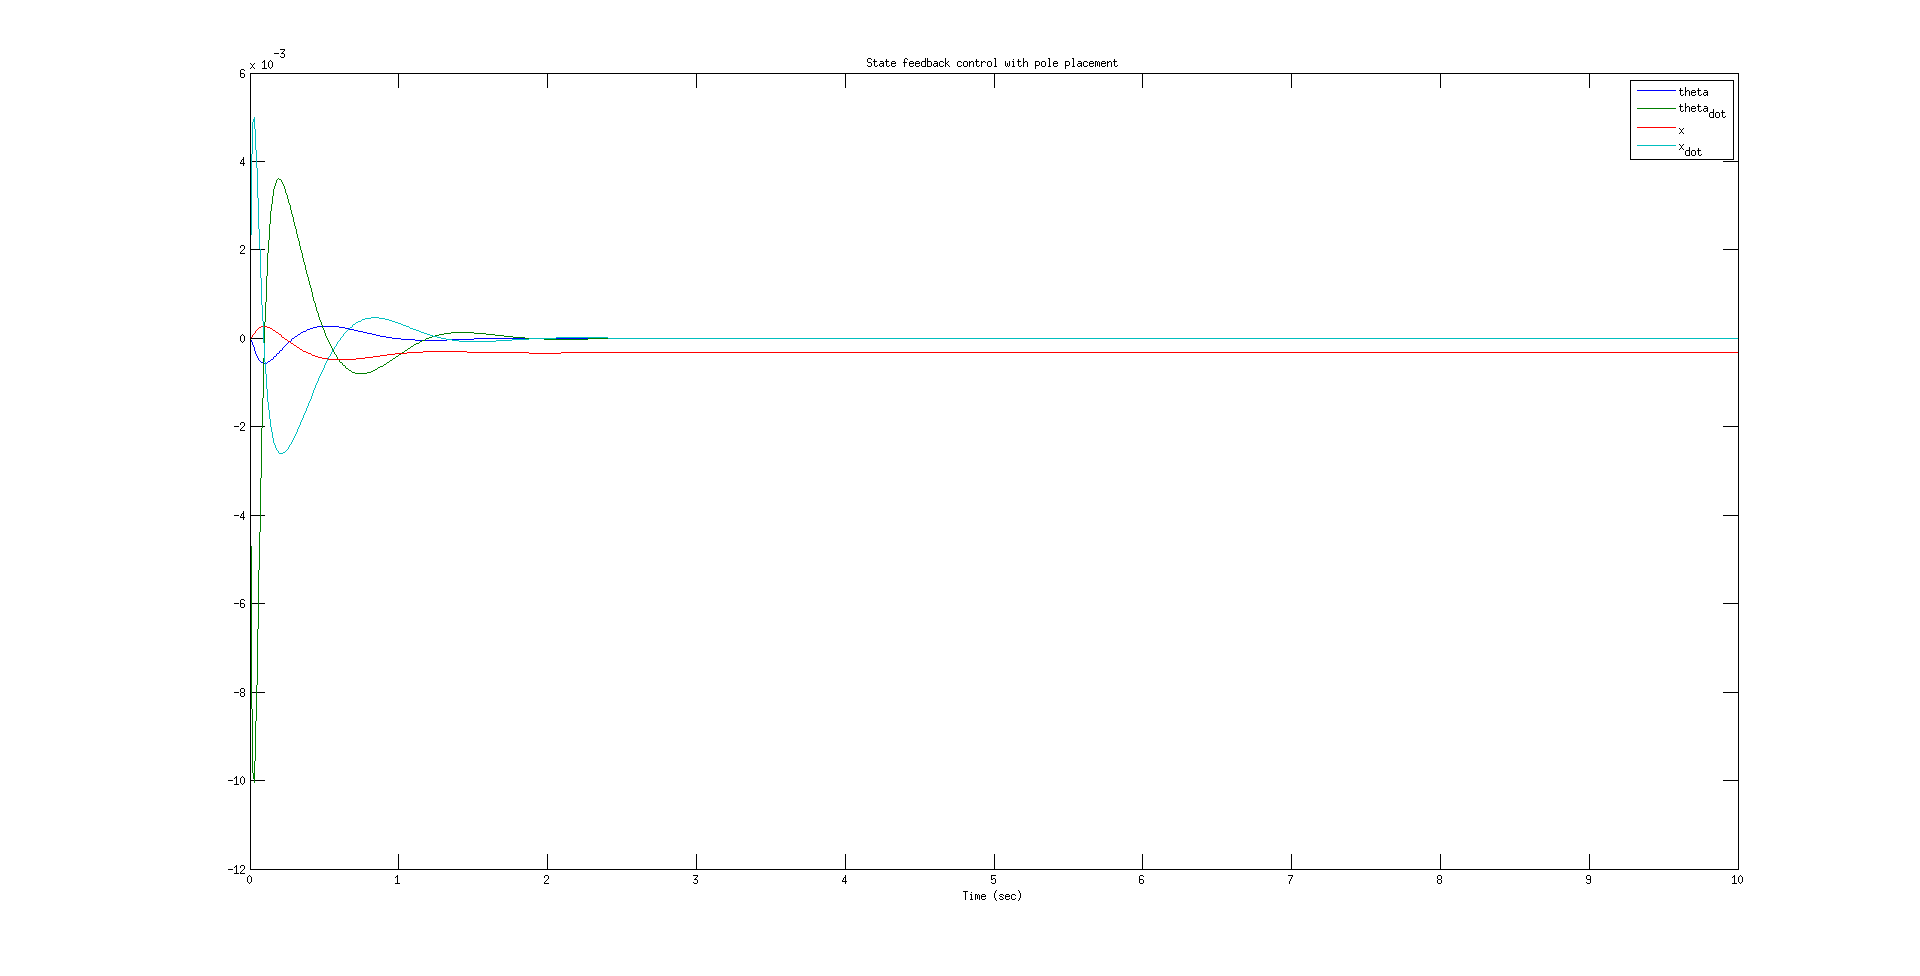
\includegraphics[width=\textwidth]{A.png}

και η επιθυμητή είσοδος $u(t) = -K x_t(t)$

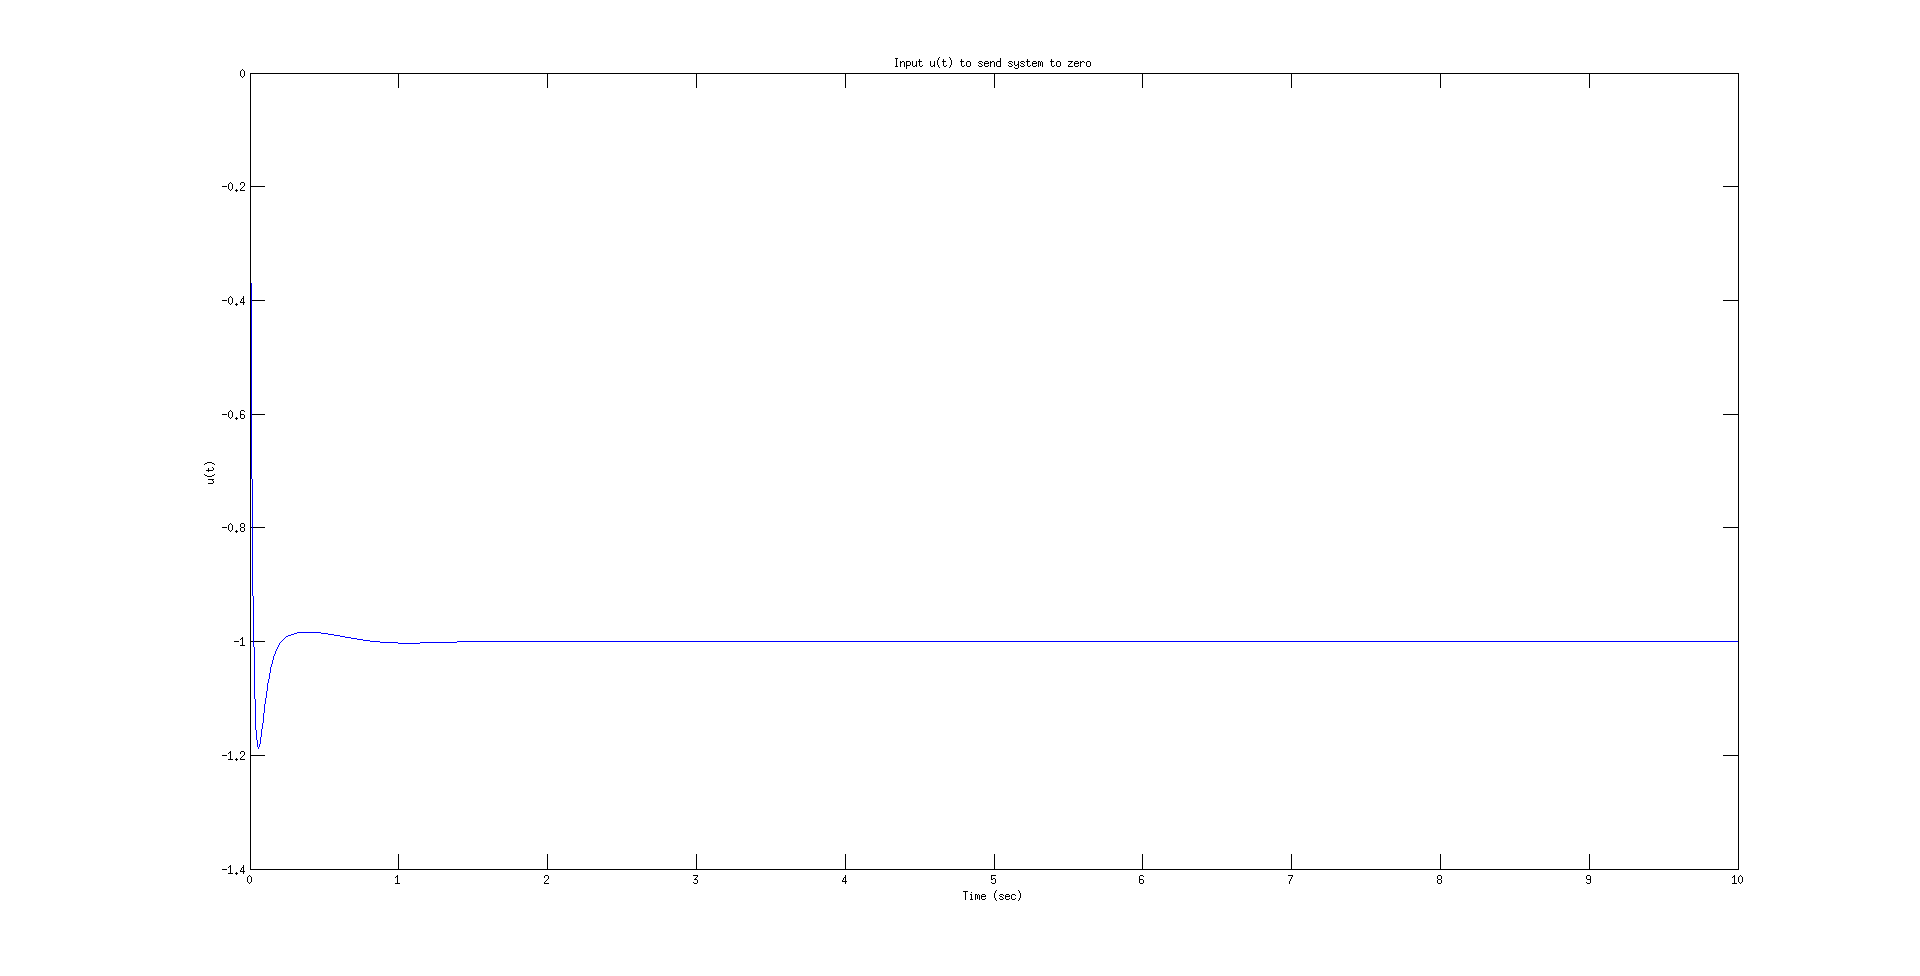
\includegraphics[width=\textwidth]{input_sf.png}


Παρατηρούμε ότι όλες οι συνιστώσες του $x_t$ έχουν απόλυτη τιμή μικρότερη του $0.015$ για $t \ge 2$.  

\paragraph{(Β) Σχεδίαση με βάση τετραγωνικό κριτήριο κόστους (LQR)} Δεδομένης της δυναμικής του συστήματος, ζητείται η εύρεση νόμου ελέγχου εισόδου $u = -Kx_t$ τέτοια ώστε $$u^*(t) = \mathrm {argmin}_u J \qquad J = \frac 1 2 \int_{0}^\infty (x_t^T (s) x_t(s) + u^2(s) ) \mathrm d s $$ όπου $J$ το τετραγωνικό κριτήριο κόστους. Η γενική μορφή του $J$ είναι $$J = \frac 1 2 \int_0^\infty (x_t^T Q x_t + u^T R u + 2x^T N u) dt$$Στη δική μας περίπτωση $Q = I, N = 0, R = 1 > 0 $. Η εύρεση του $K$ δίνεται από την αλγεβρική εξίσωση Ricatti $$A^T P + PA + PBB^TP + I = 0 \qquad P = P^T \succ 0 \qquad  K = B^T P$$ και δίνεται με χρήση της εντολής lqr στο MATLAB. Η σχεδίασή μας έδωσε τα εξής αποτελέσματα για το $K$ 
$$K =(-52.1157,  -11.5847,  -1.0000,   -2.7261)$$ 

και οι αποκρίσεις του συστήματος φαίνονται παρακάτω: 

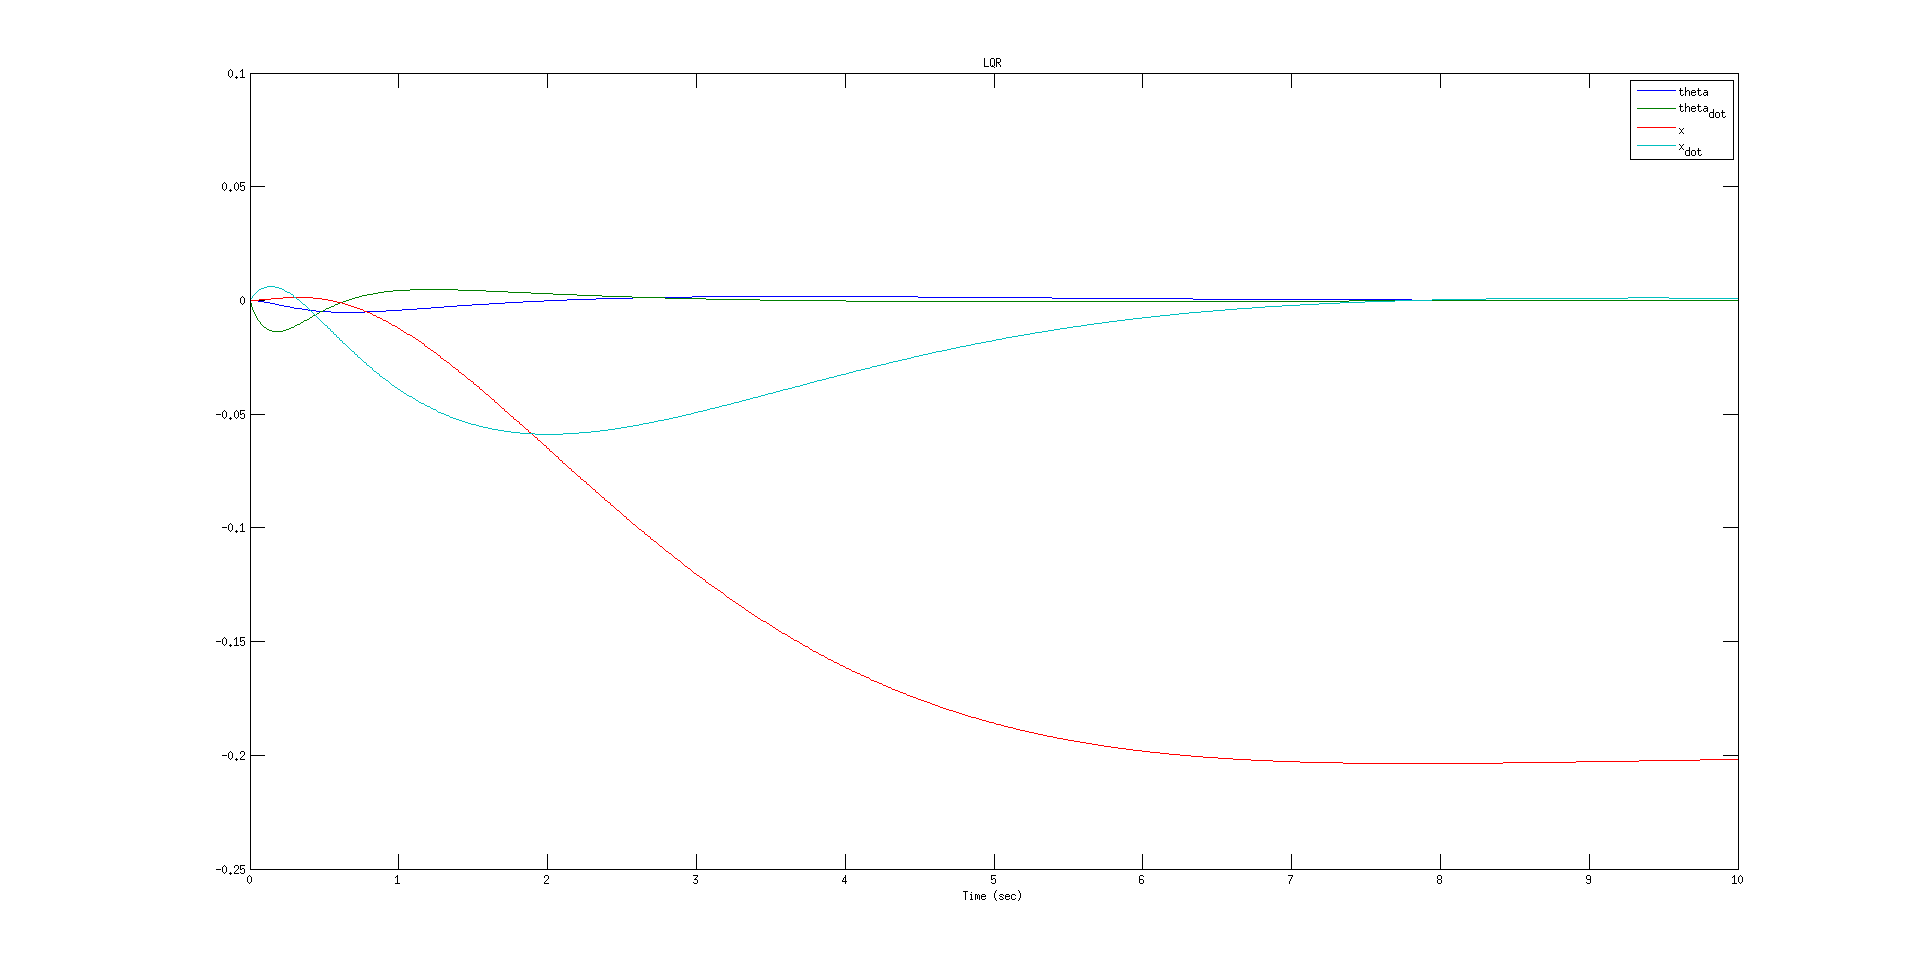
\includegraphics[width=\textwidth]{B.png}

Και ο νόμος ελέγχου:  
 
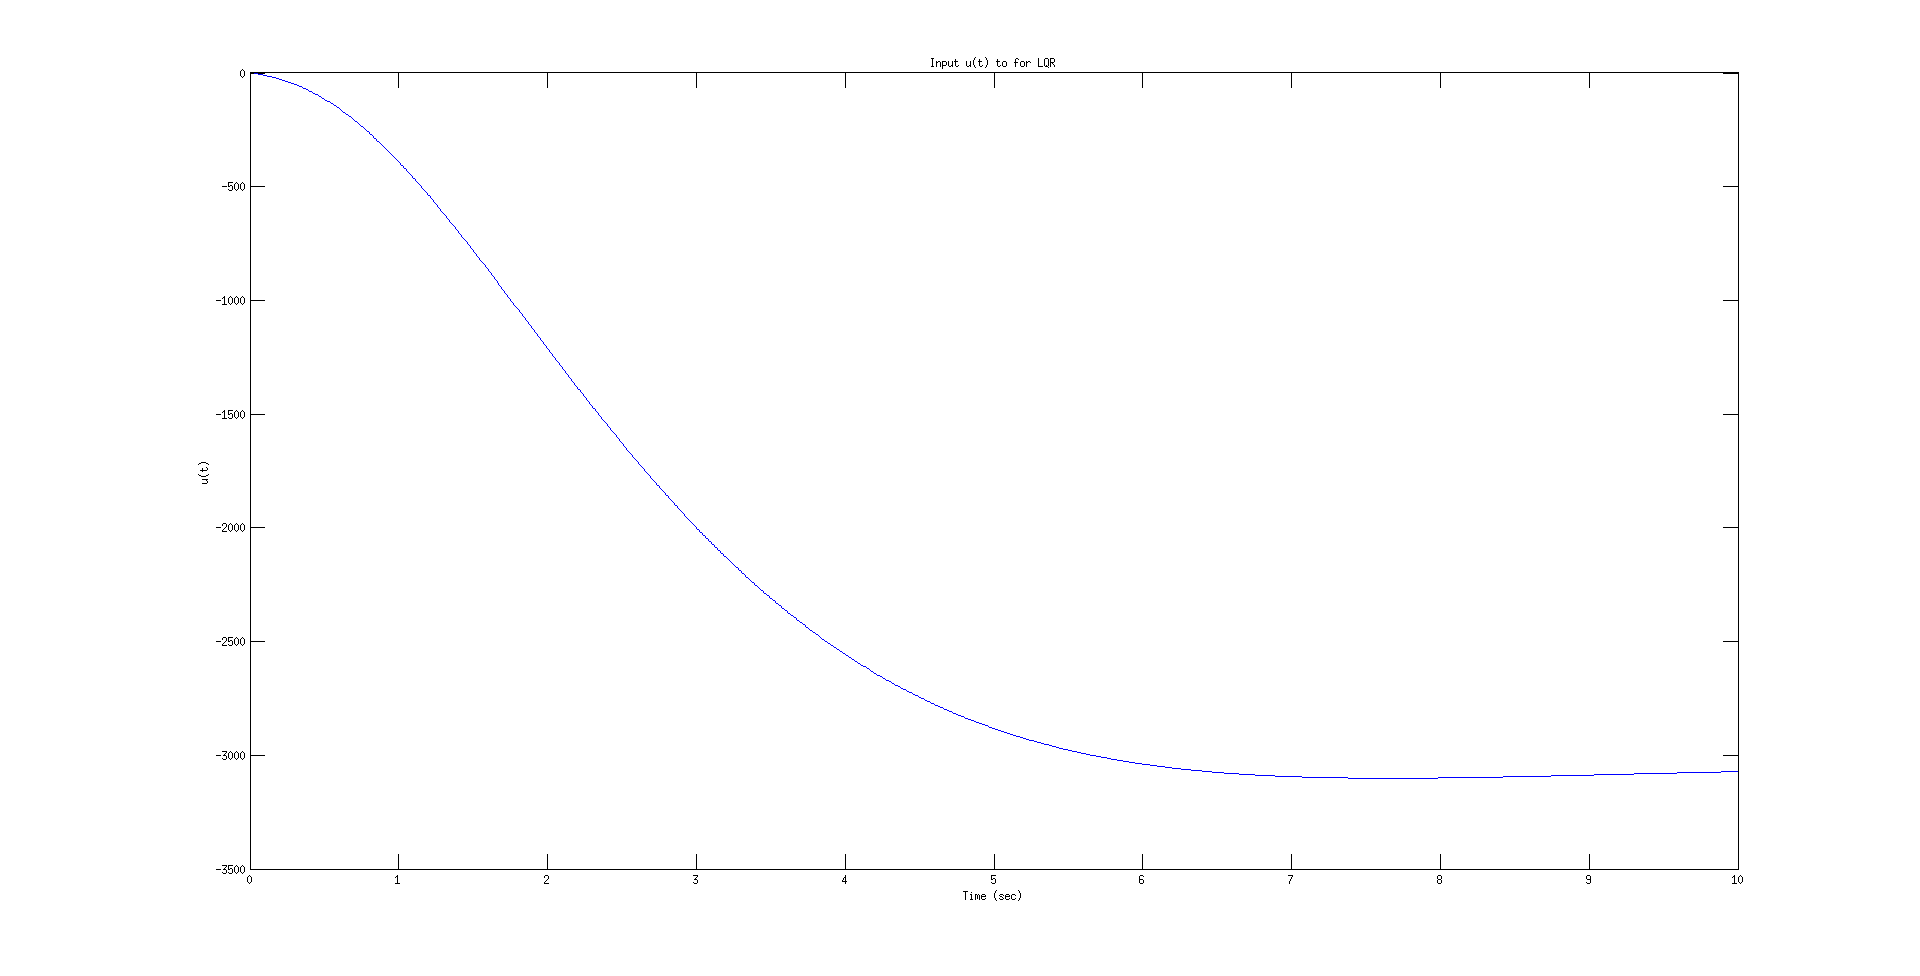
\includegraphics[width=\textwidth]{input_lqr.png}


\paragraph{(Γ) Σχεδίαση State Feedback για θέση διαφορετική της αρχικής} Έστω ότι έχουμε μια θέση $x_f$ στην οποία θέλουμε να στείλουμε το ΑΕ με state feedback. Θέλουμε η λύση της δυναμικής εξίσωσης να έχει τη μορφή $$x_t(t) = x_f + e^{(A - BK)t} x_0 \qquad \lim_{t \to \infty} \| x_t(t) - x_f \| = 0$$
Χρησιμοποιούμε νόμο ελέγχου $$u = -K(x_t -x_r) $$
Η αρχική ΔΕ γίνεται $\dot x_t = Ax_t + -BKx_t +B Κx_r$
από τη θεωρία των γραμμικών ΣΔΕ γνωρίζουμε ότι το αποτέλεσμα θα έχει μια ομογενή λύση $e^{(A - BK)t}x_0$ και μια ειδική λύση $x_p(t) = \text{σταθ}$. Με αντικατάσταση λαμβάνουμε: $$x_p = x_f = (A - BK)^{-1} BK x_r$$

Επομένως αναζητούμε $x_r$ τέτοιο ώστε $x_f = (A - BK)^{-1} BK x_r$. Έστω ότι θέλουμε να στείλουμε το αμαξάκι στη θέση -1. Διαλέγοντας $x_r = (0, 0, 1, 0)^T$ έχουμε ότι $$x_p = (0, 0, -1, 0)^T$$. Επομένως 

$$u = - K 
\begin{pmatrix}
\theta \\ \dot \theta \\ x - 1 \\ \dot x \\ 
\end{pmatrix}$$


Η απαιτούμενη ισχύς του κινητήρα είναι $$P = F \dot x = u \dot x $$ Η γραφική παράσταση της $P(t)$ είναι:

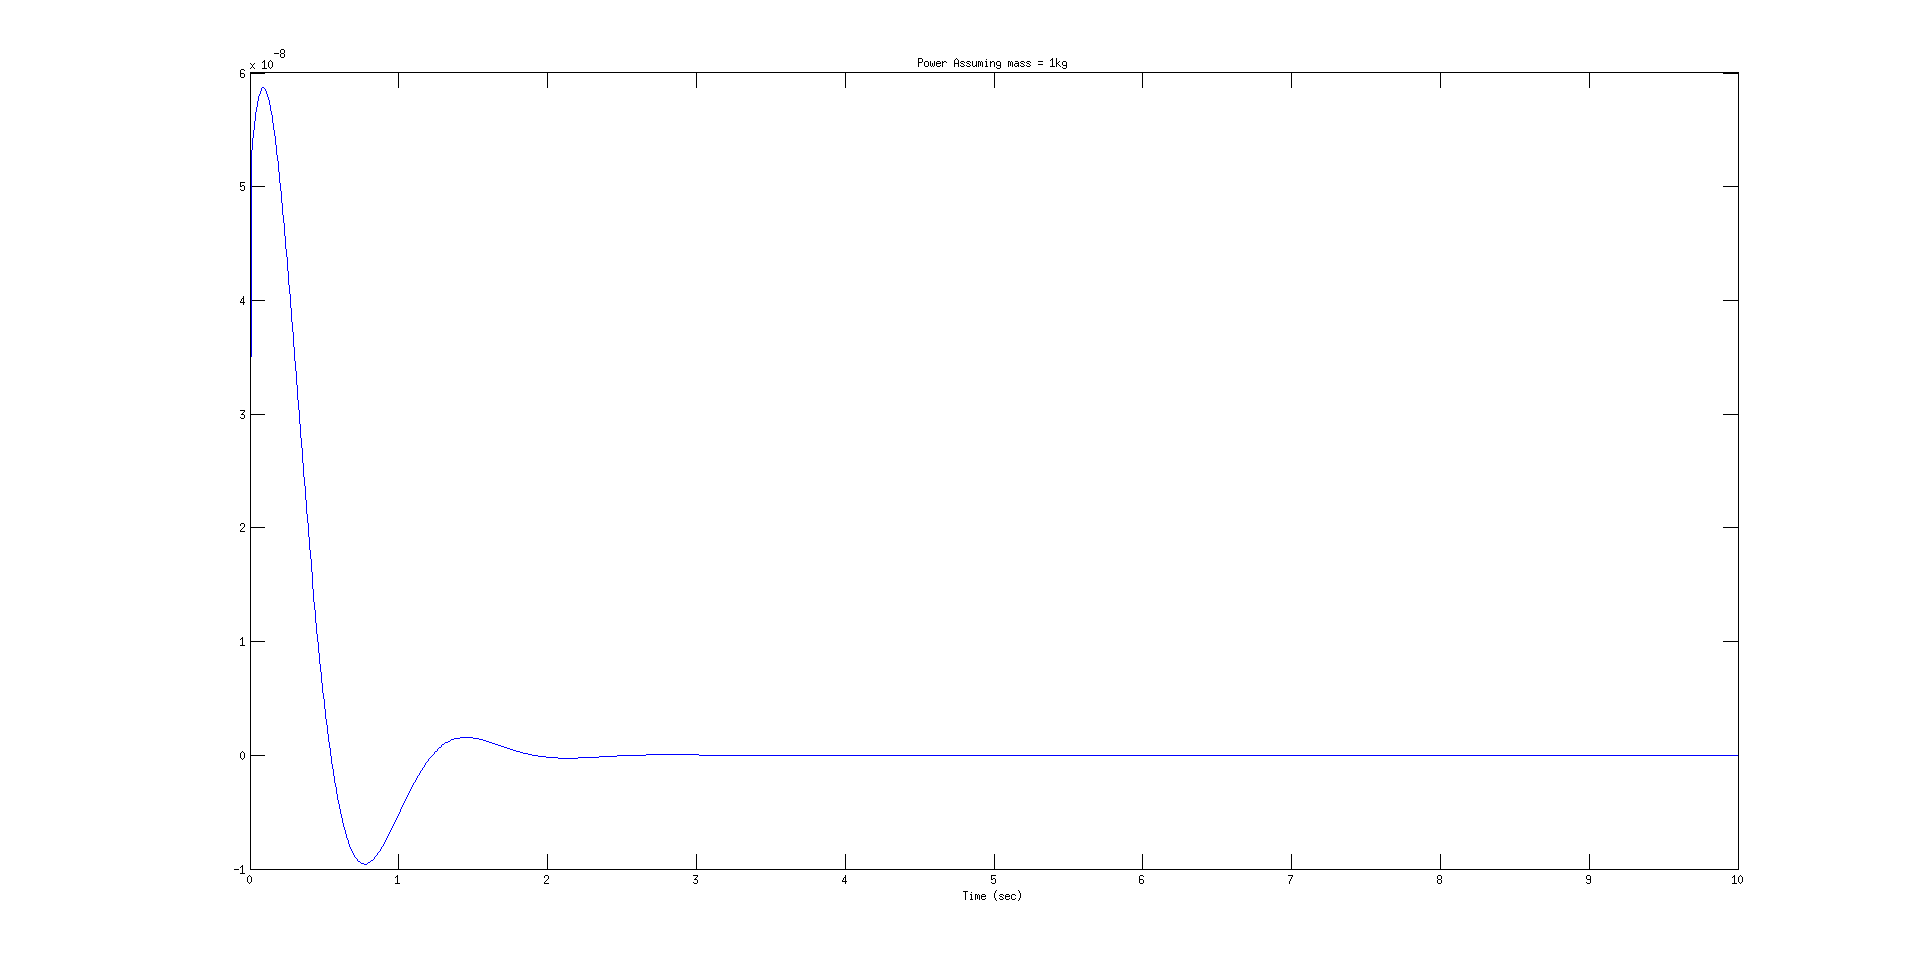
\includegraphics[width=\textwidth]{power.png}

Ενώ η είσοδος για να στείλουμε το βαγονάκι εκεί: 

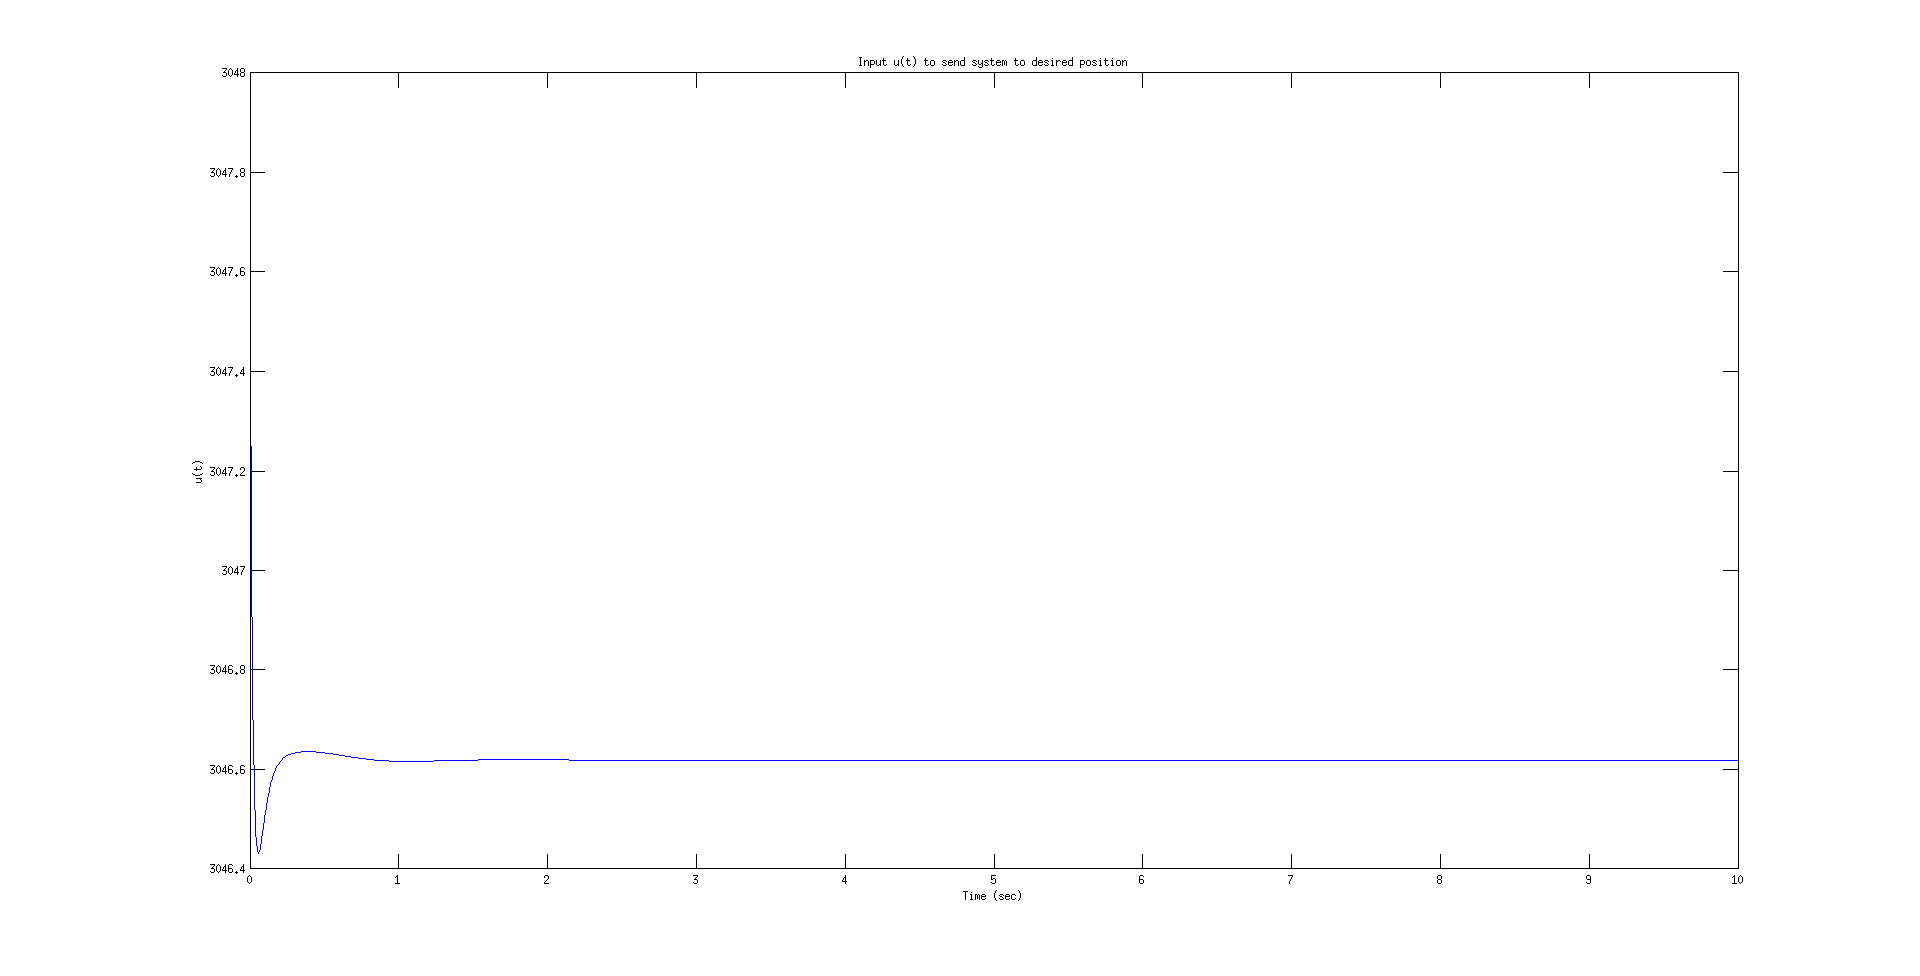
\includegraphics[width=\textwidth]{input.png}


\paragraph{(Δ) Σχεδίαση παρατηρητή πλήρους τάξης (Luenberger Observer)} Έστω ότι δεν είναι μετρήσιμο το $x_t$ αλλά το $y$. Σε αυτή την περίπτωση θα σχεδιάσουμε παρατηρητή κατάστασης πλήρους τάξης (Luenberger Observer). Θεωρούμε $\hat x_t $ εκτίμηση του διανύσματος κατάστασης $x_t$ και σφάλμα $e = x_t - \hat x_t$. Η εκτίμηση υπακούει στις δυναμικές εξισώσεις $$\dot {\hat x} = A \hat x + Bu + L (y - \hat y) \qquad \dot e = (A - LC) e $$ ενώ το $\xi = (x_t, e)^T$ υπακούει στις 

$$\dot \xi = \mathbb A \xi + \mathbb B u \qquad \text{με} \qquad \mathbb A = \begin{pmatrix}
A - BK & BK \\ \mathbb O & A - LC \\ 
\end{pmatrix}
\quad \mathbb B = \binom B {\mathbb O}$$

$$y_\xi = \mathbb C \xi  \qquad \text{με} \qquad \mathbb C = \begin{pmatrix}
C & \mathbb O
\end{pmatrix}$$

και χαρακτηρηστικό πολυώνυμο $$\chi (s) = \chi_{A-BK} (s) \chi_{A - LC} (s)$$ το οποίο υποδηλοί πως μπορούμε να διαχωρίσουμε το πρόβλημα σε 2 προβλήματα τοποθέτησης πόλων για εύρεση των gain matrices $K, L$. Με χρήση της εντολής place τοποθετούμε πόλους για την έξοδο με τον ίδιο τρόπο στις θέσεις $p_{d1}, p_{d1}^*, p_{d2}, p_{d3}$ για τη σχεδίαση του παρατηρητή πλήρους τάξης. Το αποτέλεσμα για το $L$ είναι: 

$$ L = \begin{pmatrix}
  30.3924  & -1.4081 \\ 
   28.2581 & -38.3924 \\ 
   20.3737 &  39.9409 \\
  742.5510 & 174.8646 \\
\end{pmatrix}$$

Ενώ η γραφική παράσταση για τα $x(t), \theta(t)$: 

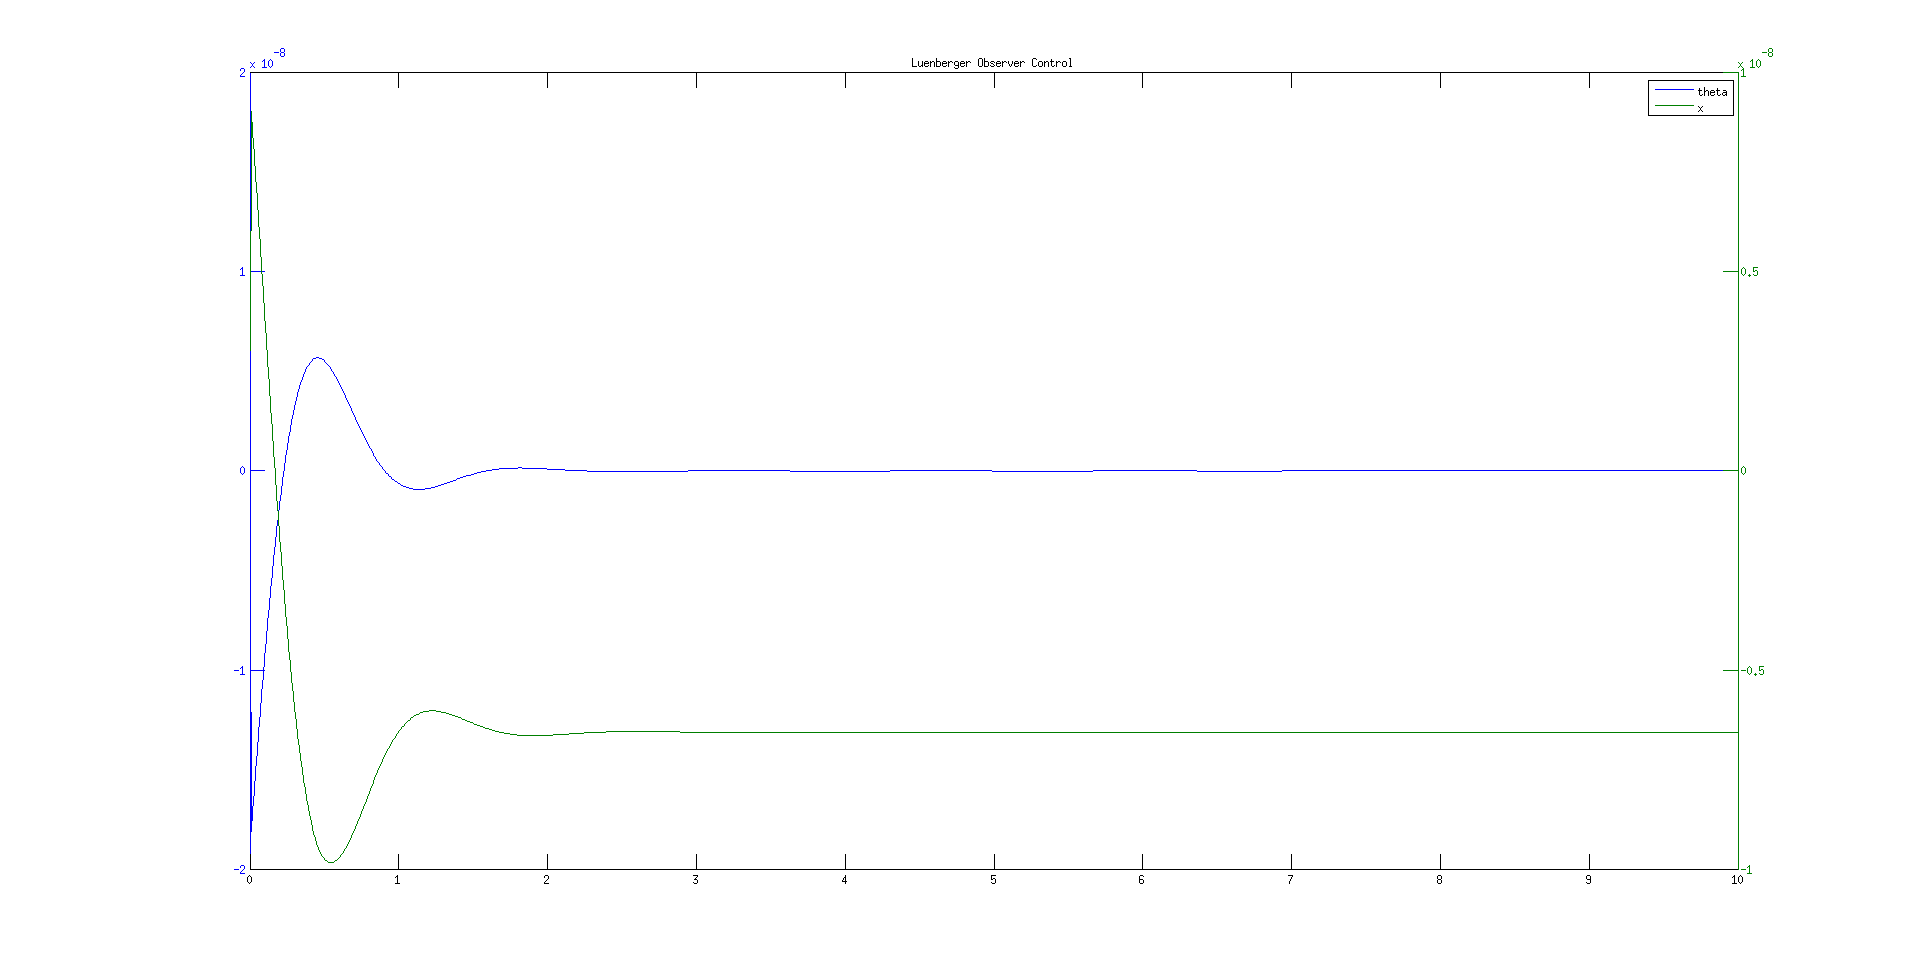
\includegraphics[width=\textwidth]{D.png}

Παρομοίως για το ερώτημα B έχουμε το ίδιο $L$ και το αποτέλεσμα είναι

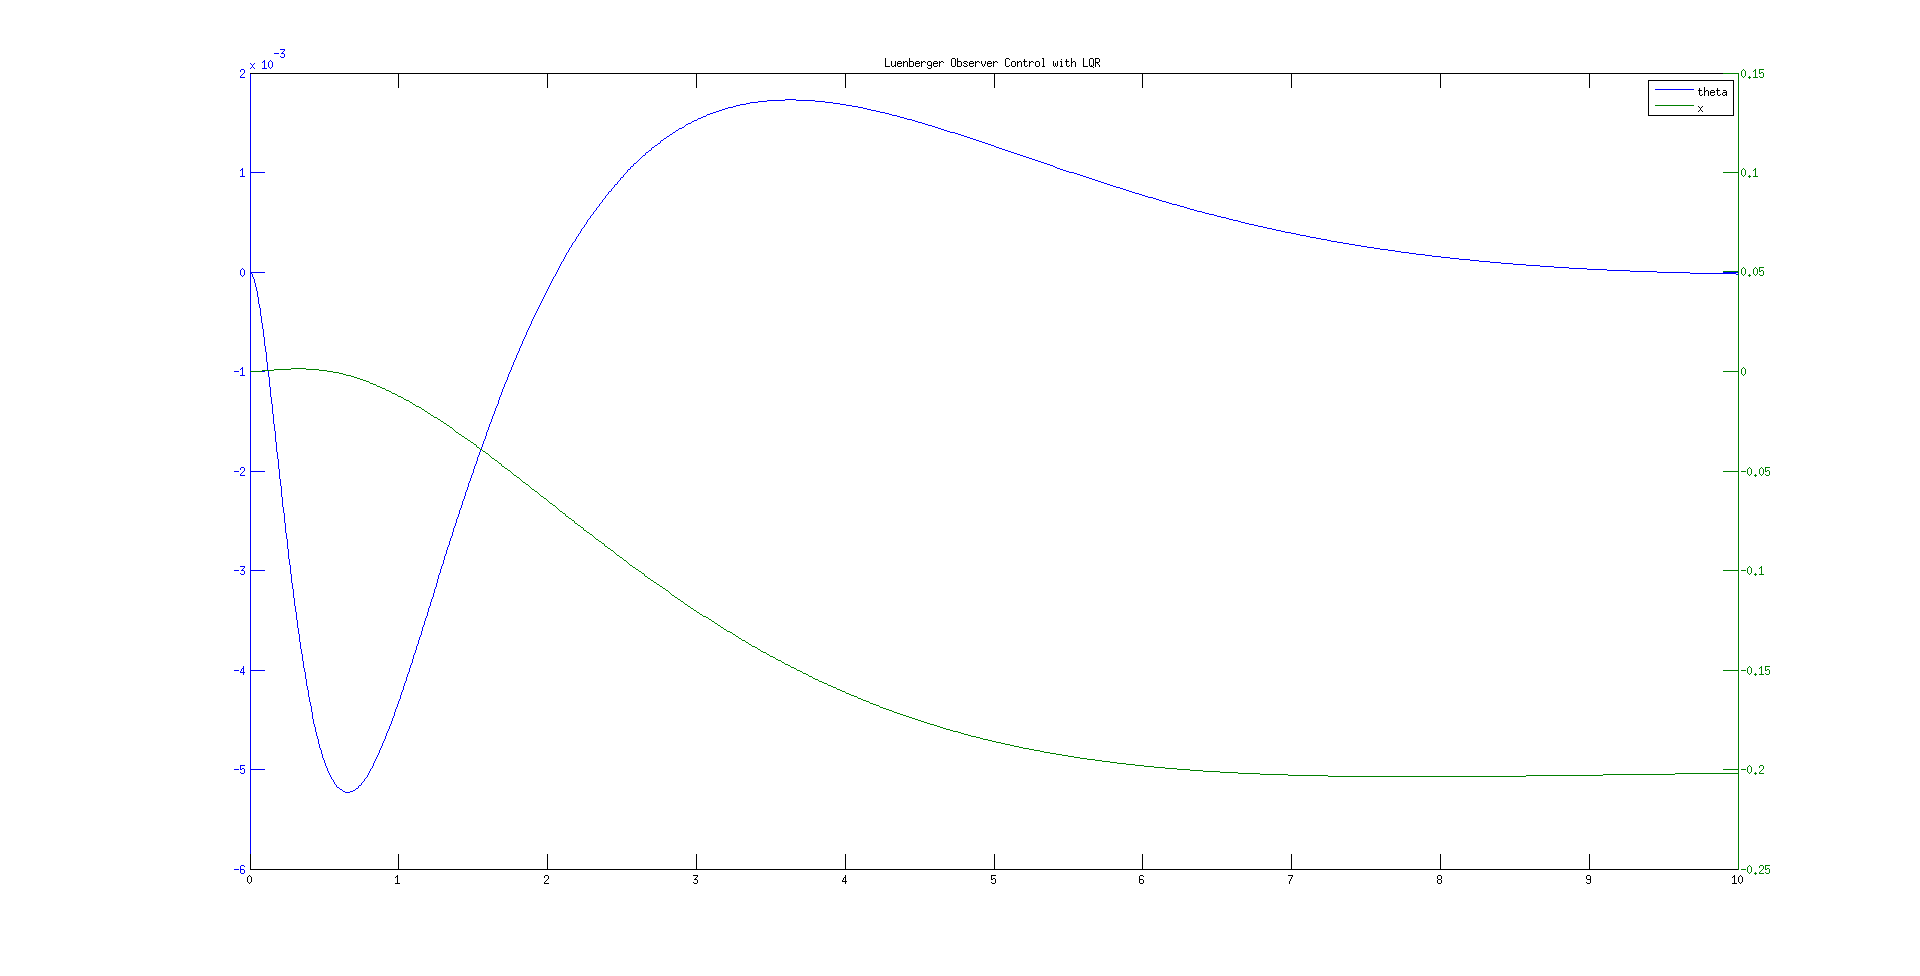
\includegraphics[width=\textwidth]{D1.png}


\paragraph{(Ε) Αλλαγή Παραμέτρων για την ίδια σχεδίαση} Αξιολογούμε τη σχεδίασή μας αν οι τιμές 20.6 και  -0.5 στον πιο πάνω πίνακα αντικατασταθούν με τις 20.9 και -0.8 αντιστοίχως. Παρατηρούμε ότι τα αποτελέσματα παραμένουν σχεδόν τα ίδια και βρίσκονται μέσα στις προδιαγραφές σχεδίασης που έχουμε θέσει. 

Για το (A)

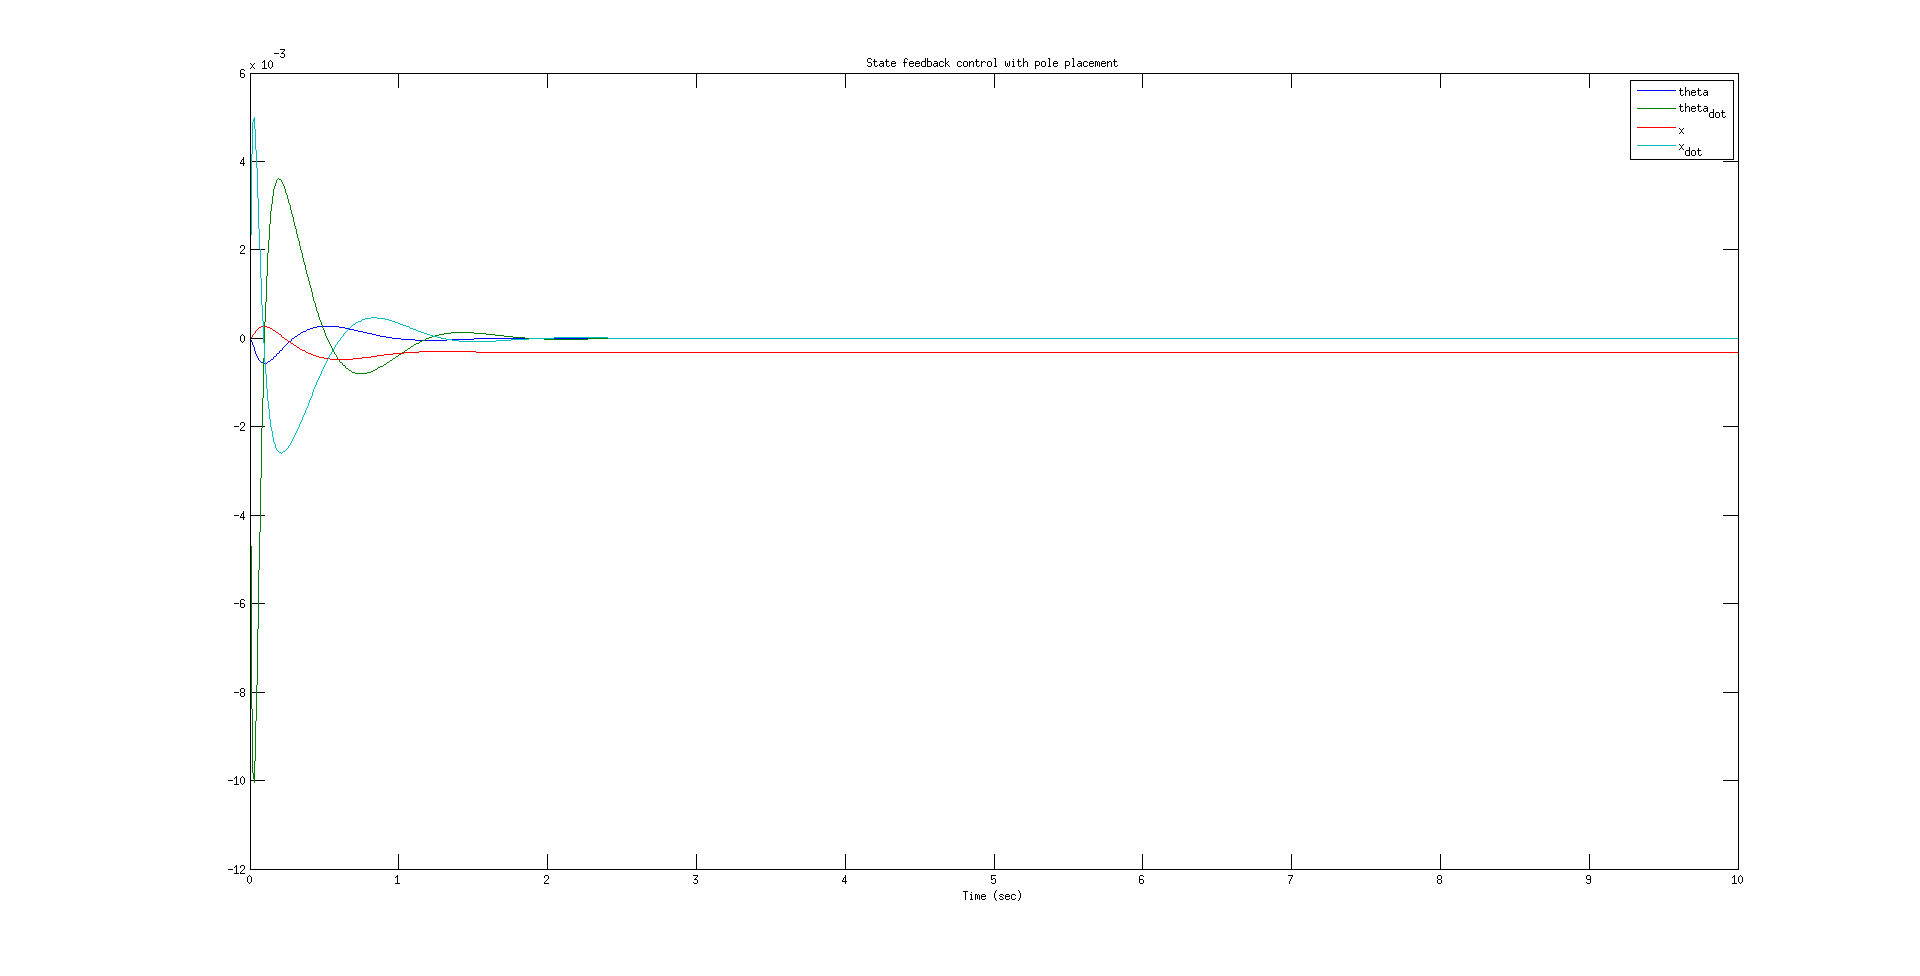
\includegraphics[width=\textwidth]{E1.png}

Για το (Β)

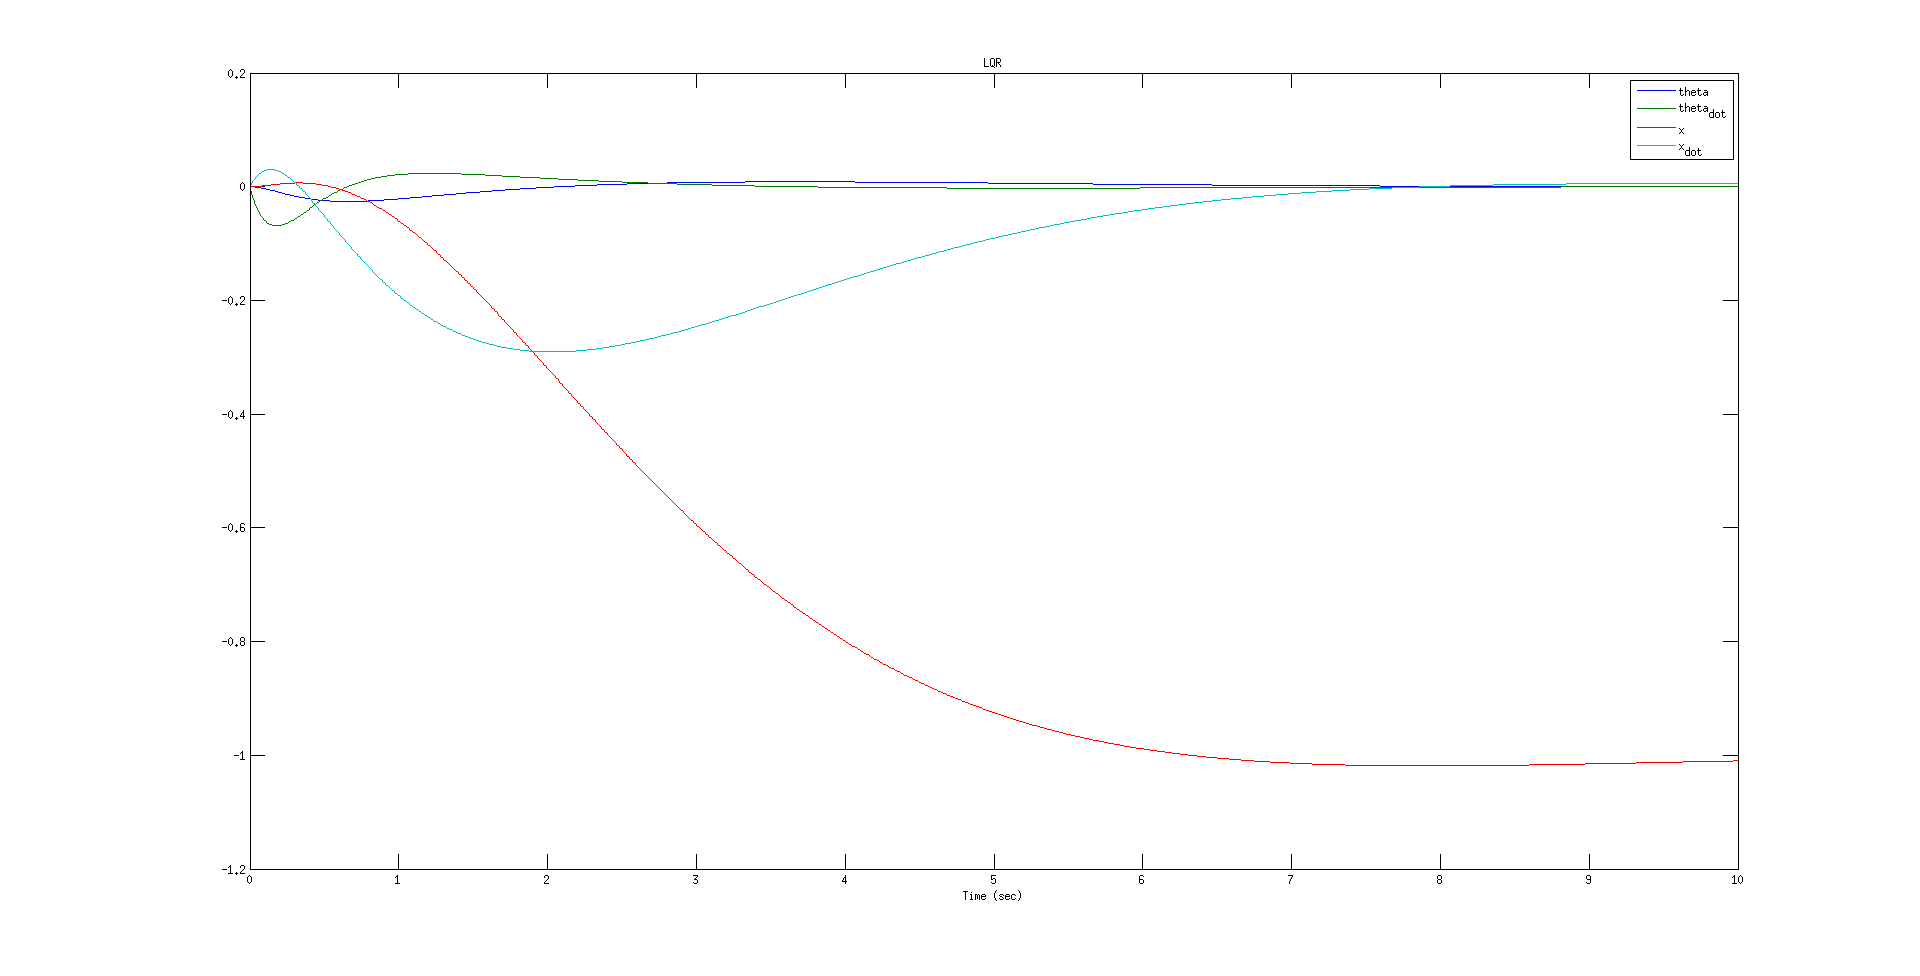
\includegraphics[width=\textwidth]{E2.png}

Για το (Γ)

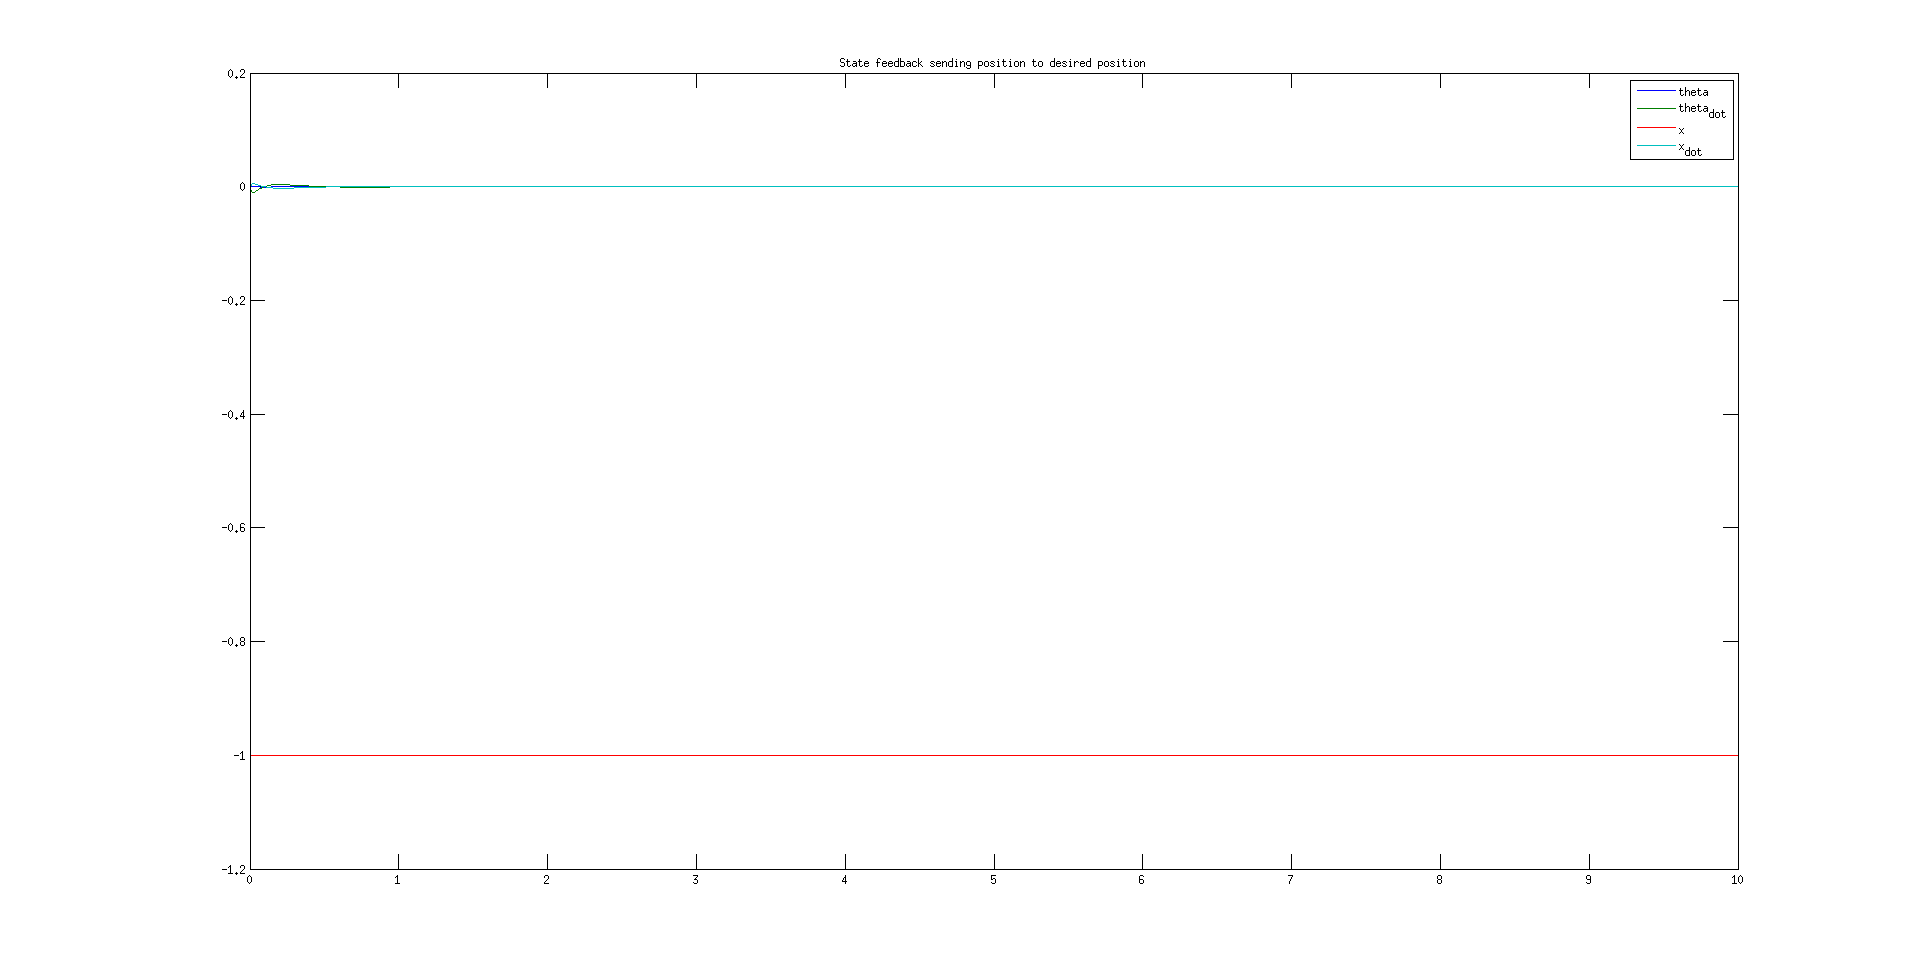
\includegraphics[width=\textwidth]{E3.png}

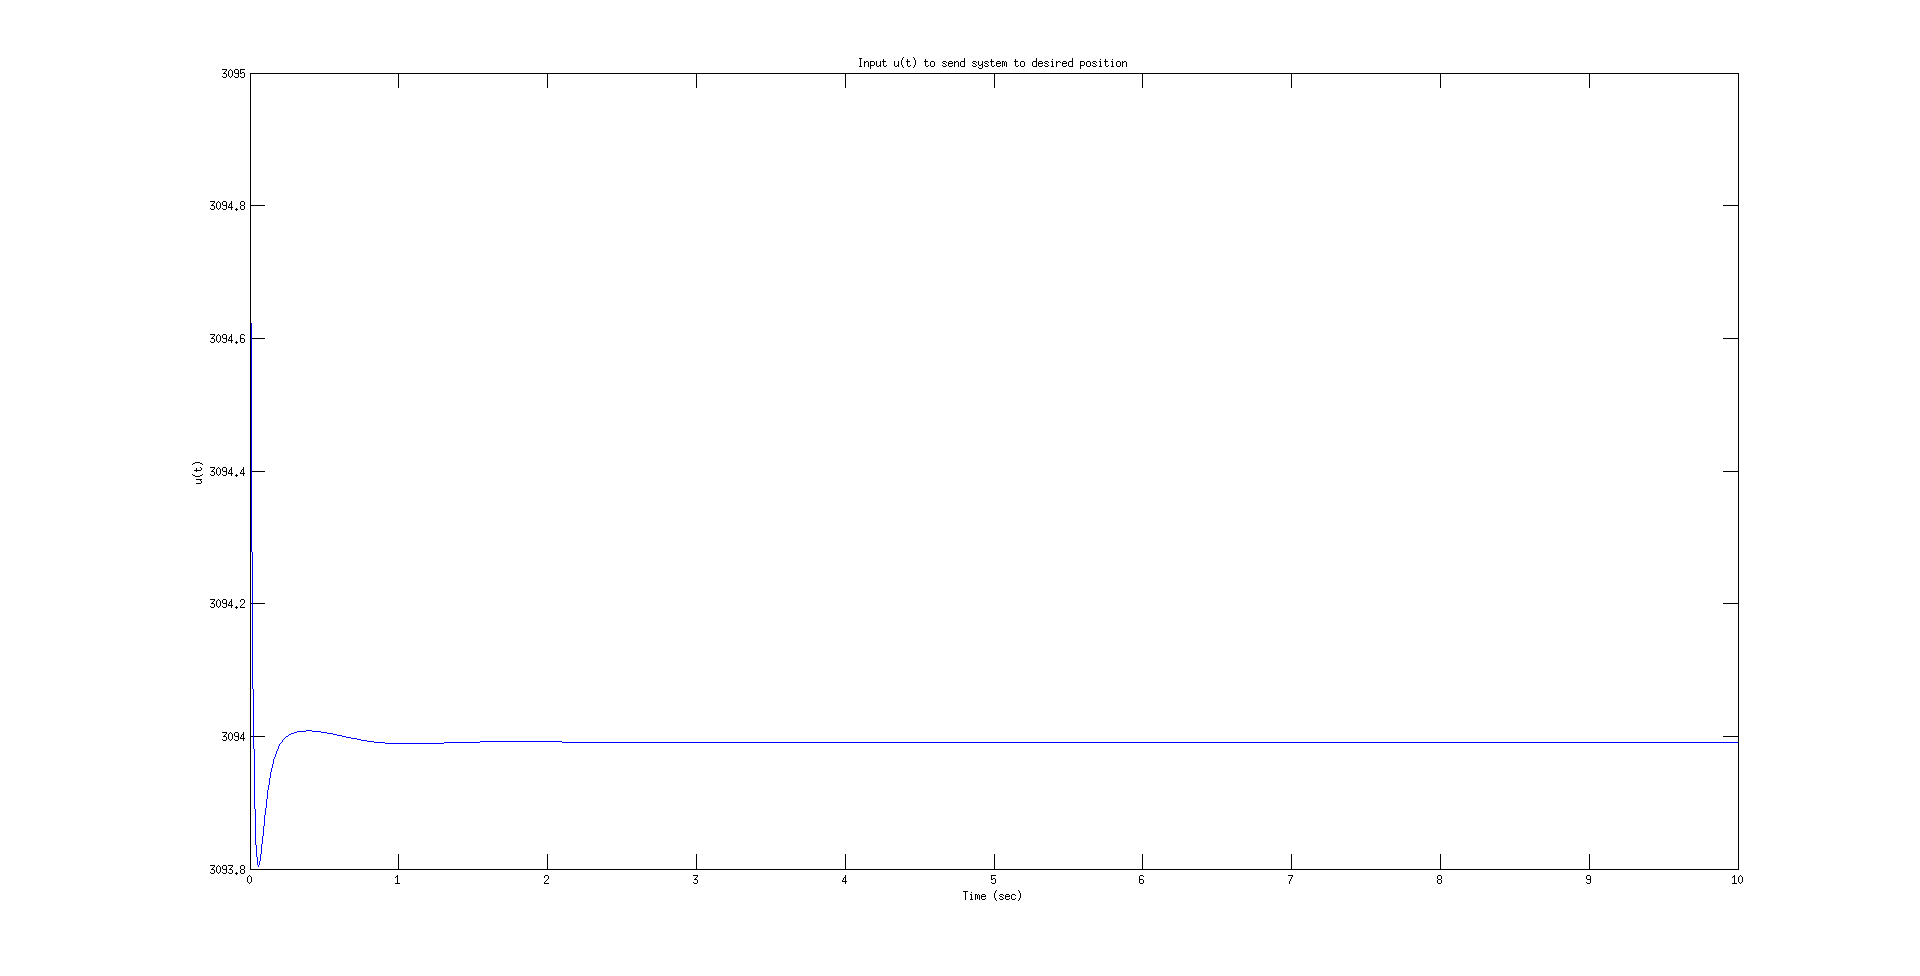
\includegraphics[width=\textwidth]{E4.png}

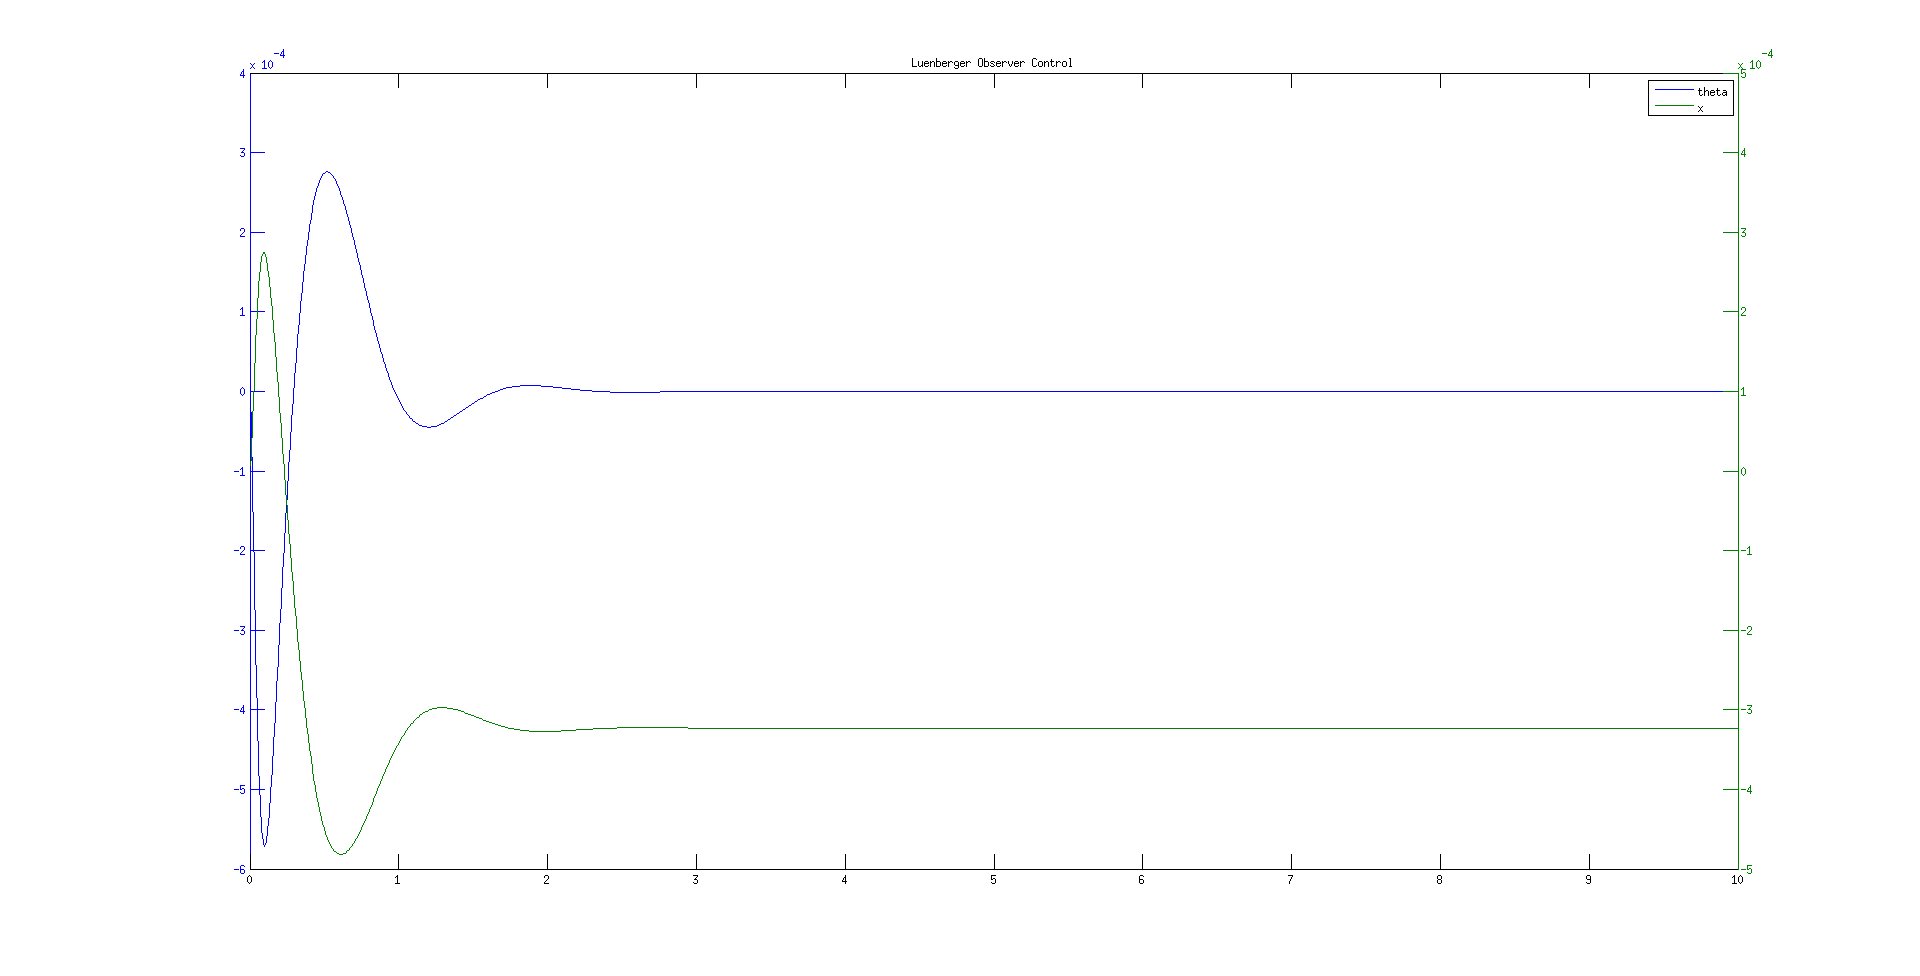
\includegraphics[width=\textwidth]{E5.png}

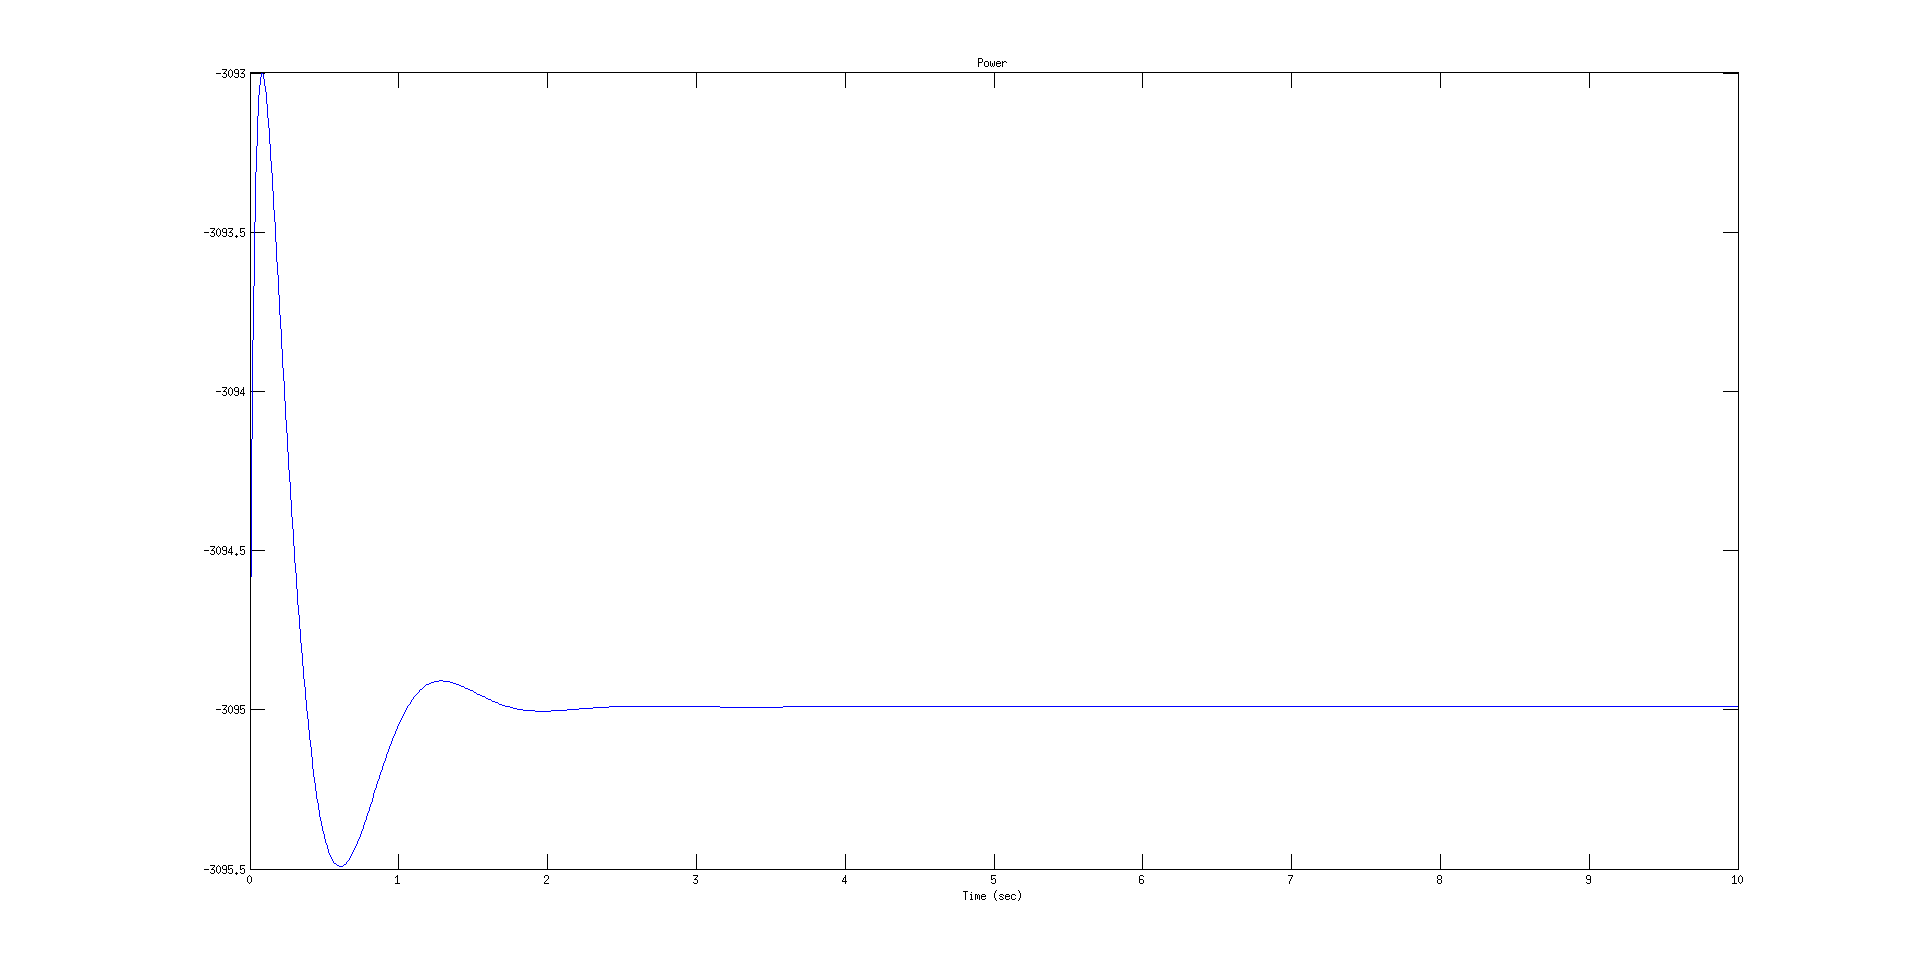
\includegraphics[width=\textwidth]{power2.png}


Για το (Δ)

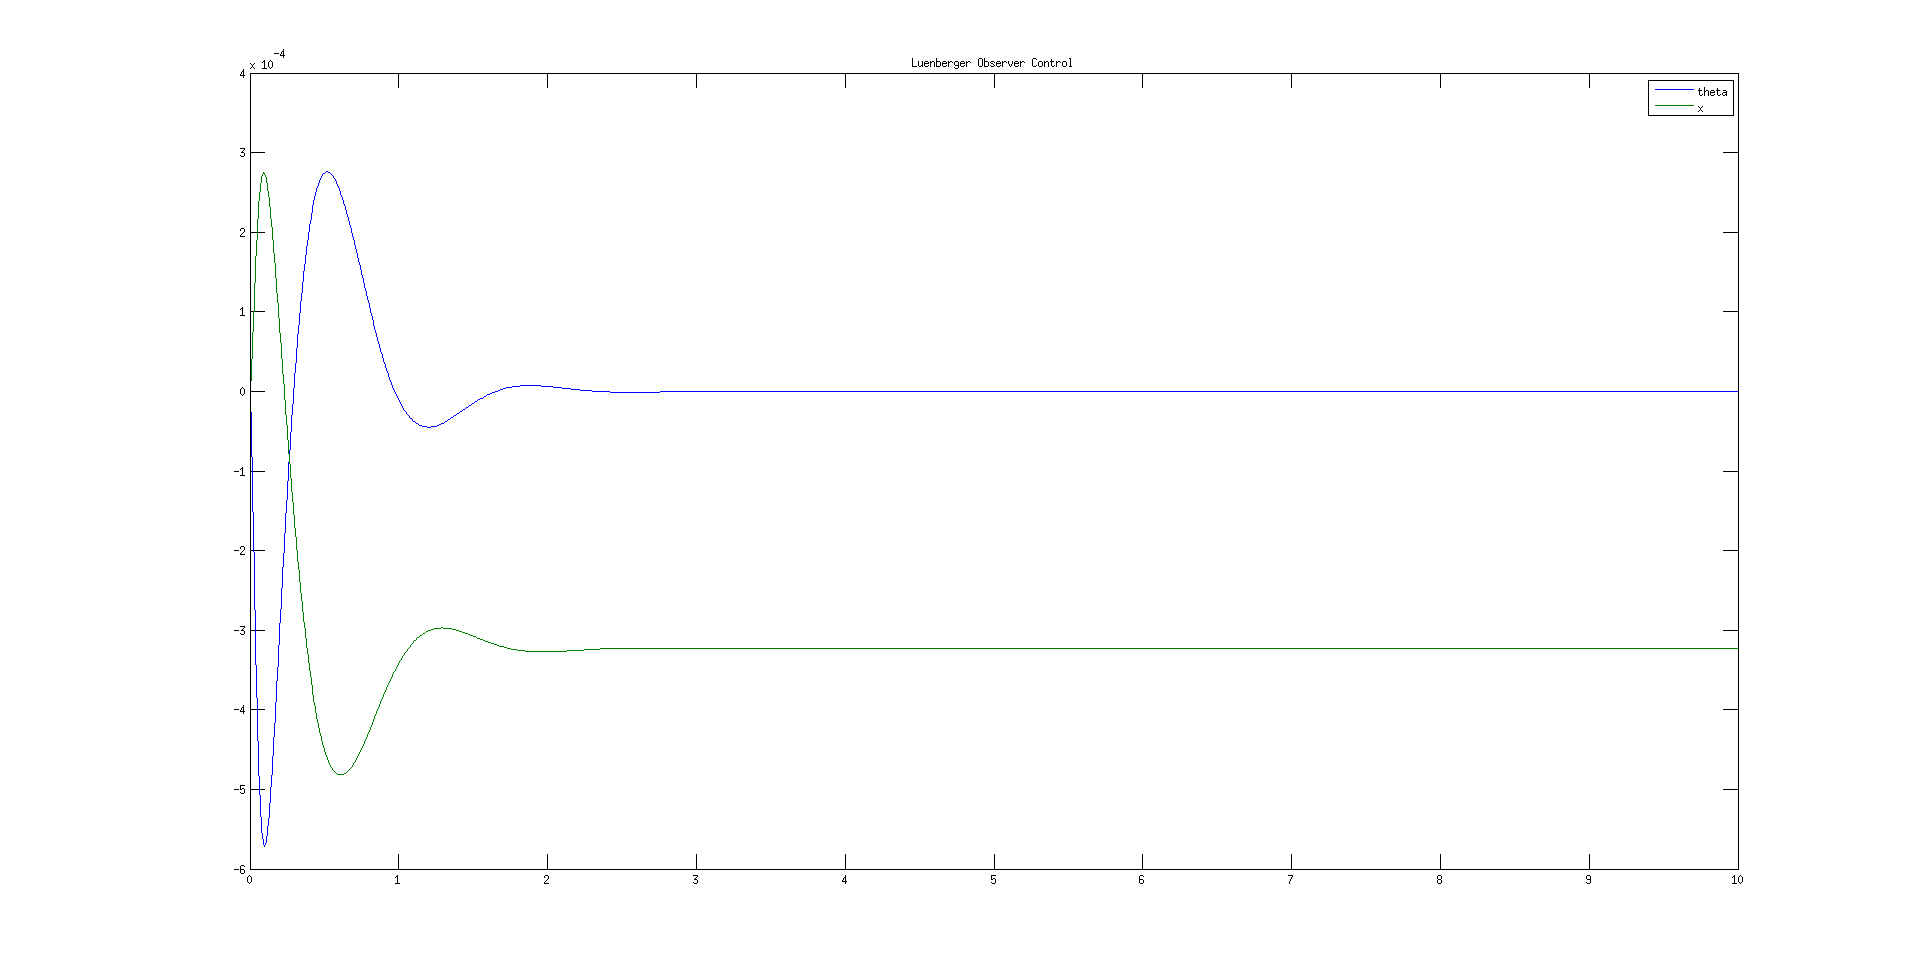
\includegraphics[width=\textwidth]{E7.png}

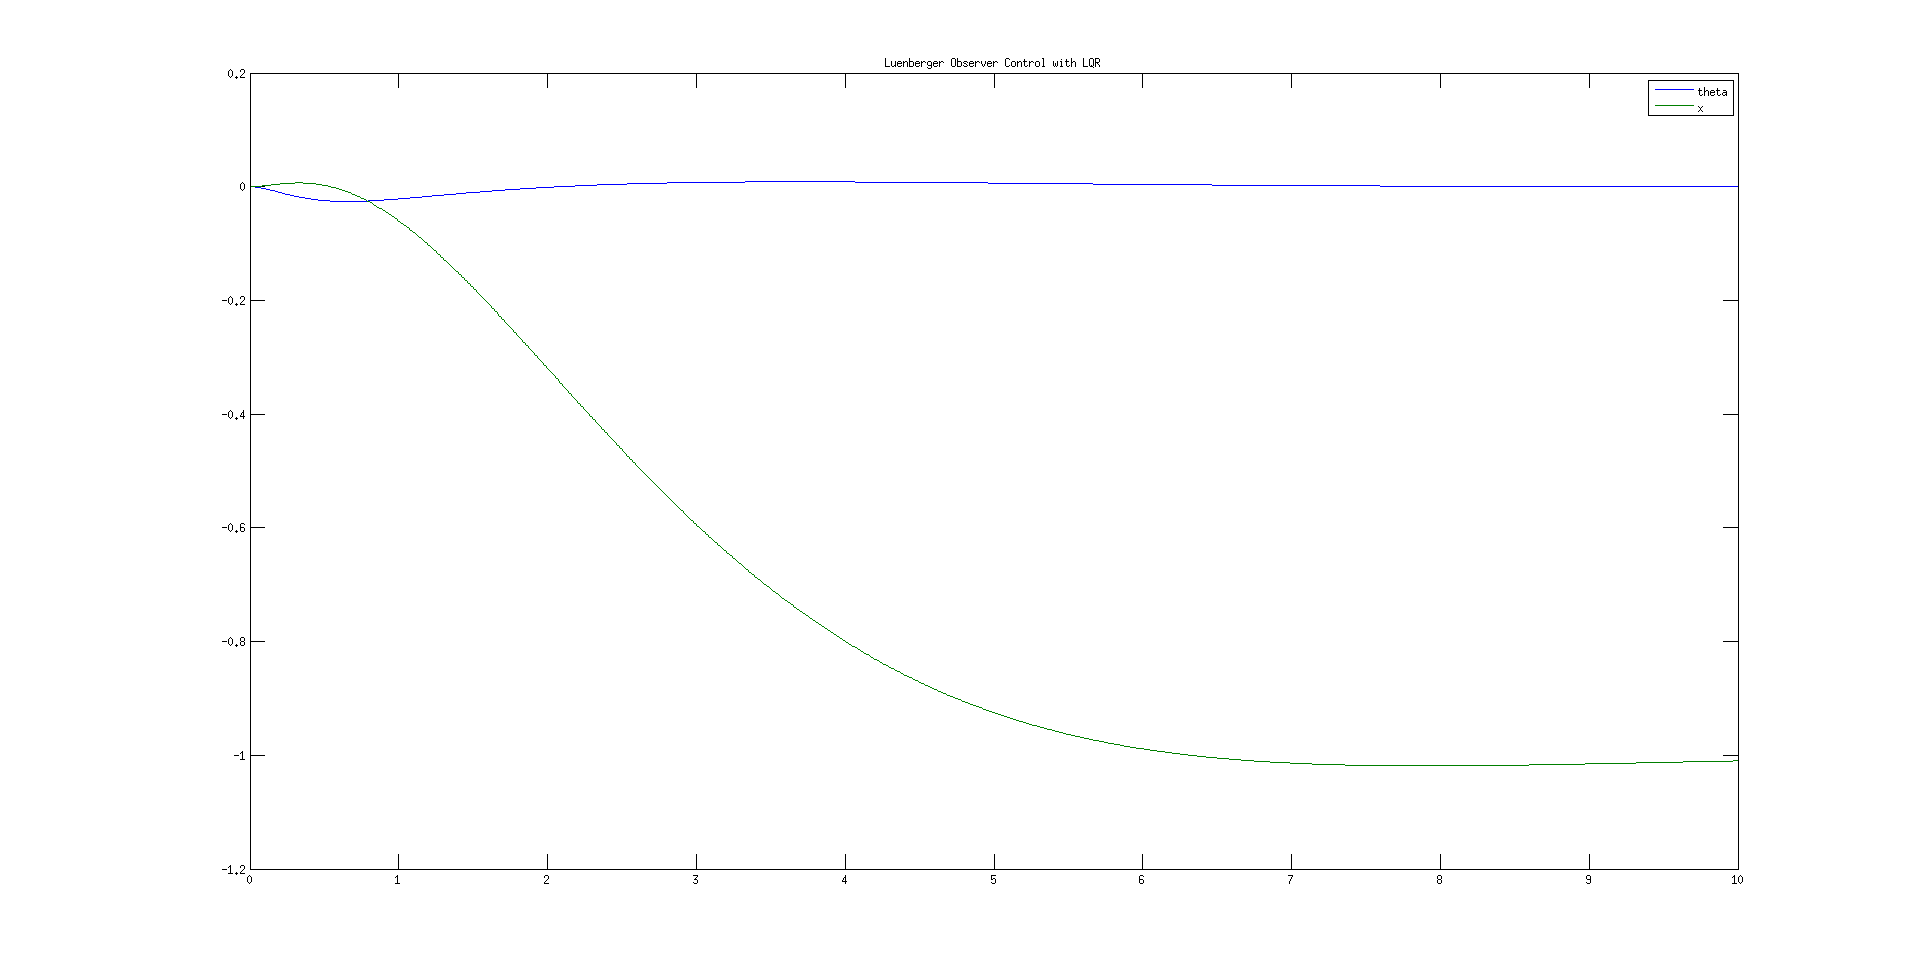
\includegraphics[width=\textwidth]{E6.png}

\section*{Πηγαίος Κώδικας}

Παρατίθεται ο κώδικας MATLAB που χρησιμοποιήσαμε για τα Α, Β, Γ, Δ. Για το τελευταίο ερώτημα αλλάζουμε τα \texttt{a, b} στις τιμές που θέλουμε.  

\begin{lstlisting}[language=Octave]
clear
close all

%% System dynamics
a = 20.6;
b = -0.5;
A = [0 1 0 0; a 0 0 0; 0 0 0 1; b 0 0 0];
B = [0; -1; 0; 0.5];
C = [1 0 0 0; 0 0 1 0];
D = [0 ; 0];
x0 = [-0.2; -0.06; 0.01; 0.3];
zeta = 0.5;
ts = 1.5;
omega_n = 4 / (zeta * ts);
t = 0:0.01:10;
r = ones(size(t));

states = {'theta' 'theta_dot' 'x' 'x_dot'};
inputs = {'u'};
outputs = {'theta'; 'x'};

sys_ss = ss(A,B,C,D,'statename',states,'inputname',inputs,'outputname',outputs);

% controllability
C_matrix = ctrb(A, B);
rank(C_matrix)

% observability
O_matrix = obsv(A, C);
rank(O_matrix);

%% A Pole Placement
omega_d = omega_n * sqrt(1 - zeta^2);
sigma = - zeta * omega_n;
p = sigma + omega_d * 1i;

poles = [p conj(p) -30 -35];
Kp = place(A, B, poles);

sys_cl_sf = ss(A - B * Kp, B, C, D,'statename',states,'inputname',inputs,'outputname',outputs);

figure;
[y_sf,t,x_sf]=lsim(sys_cl_sf,r,t);
plot(t, x_sf);
legend('theta', 'theta_{dot}', 'x', 'x_{dot}');
title('State feedback control with pole placement');
xlabel('Time (sec)');

figure;
u_sf = - Kp * x_sf';
plot(t, u_sf);
title('Input u(t) to send system to zero');
xlabel('Time (sec)');
ylabel('u(t)');



%% B LQR 
Q = eye(4);
R = 1;
[K, S, e] = lqr(A,B,Q,R);
N = 0;

newA = A - B * K;

states = {'theta' 'theta_dot' 'x' 'x_dot'};
inputs = {'r'};
outputs = {'theta'; 'x'};

sys_cl_lqr = ss(newA, B, C, D,'statename',states,'inputname',inputs,'outputname',outputs);

figure;
[y,t,x_lqr]=lsim(sys_cl_lqr,r,t);
plot(t, x_lqr);
legend('theta', 'theta_{dot}', 'x', 'x_{dot}');
xlabel('Time (sec)');
title('LQR');
 
u_lqr = - Kp * x_lqr';
figure;
plot(t, u_lqr);
title('Input u(t) to for LQR');
xlabel('Time (sec)');
ylabel('u(t)');


%% C Send the system to desired position
xr = [0 0 1 0]';
xf = inv(A - B * Kp) * B * Kp * xr;
u = -Kp * x_sf' - Kp * xr;
figure;
plot(t, u);
title('Input u(t) to send system to desired position');
xlabel('Time (sec)');
ylabel('u(t)');

x_new = x_sf;
[rown, coln] = size(x_sf);
for j = 1 : rown
    x_new(j, :) = x_new(j, :) + xf';
end;
figure;
plot(t, x_new);
title('State feedback sending position to desired position');
legend('theta', 'theta_{dot}', 'x', 'x_{dot}');

x_new_dot = A * x_new' + B * u;
velocity = x_new(:, 3);
acceleration = x_new(:, 4);
mass = 1;
power = u' .* velocity;

figure;
plot(t, power);
title('Power');
xlabel('Time (sec)');



%% D Luenberger observer

% State Feedback
L = place(A', C', poles)';
A_ = [(A-B*Kp) (B*Kp); zeros(size(A)) (A-L*C)];
B_ = [B; zeros(size(B))];
C_ = [C zeros(size(C))];
D_ = [0; 0];

states = {'theta' 'theta_dot' 'x' 'x_dot' 'e1' 'e2' 'e3' 'e4'};
inputs = {'r'};

sys_est_cl = ss(A_,B_,C_,D_,'statename',states,'inputname',inputs,'outputname',outputs);

figure;
[y,t,x]=lsim(sys_est_cl,r,t);
plot(t, y);
title('Luenberger Observer Control')
legend('theta', 'x');

% Luenberger with LQR 
A__ = [(A-B*K) (B*K); zeros(size(A)) (A-L*C)];

states = {'theta' 'theta_dot' 'x' 'x_dot' 'e1' 'e2' 'e3' 'e4'};
inputs = {'r'};

sys_est_cl = ss(A__,B_,C_,D_,'statename',states,'inputname',inputs,'outputname',outputs);

figure;
[y,t,x]=lsim(sys_est_cl,r,t);
plot(t, y);
title('Luenberger Observer Control with LQR')
legend('theta', 'x');
\end{lstlisting}




\section*{Αναφορές}

\noindent [1] Dorf, Richard C., and Robert H. Bishop. Modern control systems. Pearson, 2011.

\noindent [2] Paraskevopoulos, P. N. Modern control engineering. CRC Press, 2001.

\noindent [3] Ogata, Katsuhiko, and Yanjuan Yang. Modern control engineering. Vol. 4. India: Prentice hall, 2002.

\end{document}



